\chapter{Теория вероятностей}
\pagenumbering{arabic}

\section{Вероятностное пространство. Операции над событиями. Свойства вероятности}
\begin{defn}
	\textit{Пространство элементарных исходов} $\Omega$~--- любое непустое множество, содержащее все возможные результаты случайного эксперимента.
	Элементы $\omega \in \Omega$~--- \textit{элементарные исходы}.
\end{defn}

\begin{defn}
	\textit{Алгебра} $\Alg$~--- множество подмножеств $\Omega$, обладающее следующими свойствами:
	
	\begin{enumerate}
		\item 
		      $\Omega \in \Alg$;
		\item 
		      $A \in \Alg \implies \overline{A} \in \Alg$; \footnote{Здесь и в дальнейшем $\overline{A} \equiv \Omega \setminus A$~--- \textit{дополнение} к $A$.}
		\item 
		      $A, B \in \Alg \implies A \cup B \in \Alg$ 
		      (по индукции: $A_1, A_2, \ldots, A_n \in \Alg \implies \\ \implies \bigcup\limits_{i=1}^n A_i \in \Alg$).
	\end{enumerate}
\end{defn}

\begin{rmrk}
	Если $A, B \in \Alg$, то $A \cap B \equiv \overline{\overline{A} \cup \overline{B}} \in \Alg$.
\end{rmrk}

\begin{defn}
	$\sigma \textit{{-алгебра~}} \SigAlg$~--- множество подмножеств $\Omega$, обладающее следующими свойствами:
	
	\begin{enumerate}
		\item 
		      $\Omega \in \SigAlg$;
		\item 
		      $A \in \SigAlg \implies \overline{A} \in \SigAlg$;
		\item 
		      $A_1, A_2,\ldots, A_n,\ldots \in \SigAlg \implies \bigcup\limits_{i=1}^\infty A_i \in \SigAlg$.
	\end{enumerate}
\end{defn}
\begin{exmp}
	Множество всех подмножеств $2^{\Omega}$ и множество $\{\varnothing, \Omega\}$~--- $\sigma$-алгебры над $\Omega$.
\end{exmp}
\begin{rmrk}
	Любая $\sigma \text{-алгебра}$ является алгеброй. 
	Первые два пункта определений идентичны, рассмотрим третий. 
	Для любой конечной последовательности $A_1, A_2,\ldots, A_n \in \Alg$ составим соответствующую счётную последовательность $A_1, A_2, \ldots, A_n, A_{n+1}=\varnothing, A_{n+2}=\varnothing,\ldots \in \Alg$. 
	Пустое множество $\varnothing$ принадлежит $\sigma$-алгебре (т.к. $\varnothing = \overline{\Omega}$).
	По определению $\sigma \text{-алгебры}$: $\bigcup\limits_{i=1}^\infty A_i \in \SigAlg \implies \bigcup\limits_{i=1}^n A_i \in \SigAlg$, следовательно, выполнен третий пункт определения алгебры.
\end{rmrk}

\begin{defn}
	\textit{Случайное событие} $A$~--- элемент $\sigma \text{-алгебры~} \SigAlg$, т.е. некоторое подмножество элементарных исходов. 
	$A=\varnothing$~---\textit{невозможное событие}, $A=\Omega$~--- \textit{достоверное событие}. 
	Событие $\overline{A}$~--- \textit{противоположное} $A$, т.е. происходит тогда и только тогда, когда не происходит $A$.
	
	Операции над событиями:
	
	\begin{compactlist}
		\item 
		\textit{Объединение} $A \cup B$~--- происходит или $A$, или $B$, или оба вместе.
		\item 
		\textit{Пересечение} $A \cap B$ (или $AB$)~--- происходят и $A$ и $B$ вместе. Если $AB = \varnothing$, то события $A$ и $B$ называются \textit{несовместными}.
		\item 
		\textit{Разность} $A \setminus B$~--- происходит $A$ и не происходит $B$.
		\item 
		\textit{Симметрическая разность} $A \triangle B$~--- либо происходит $A$ и не происходит $B$, либо происходит $B$ и не происходит $A$.
	\end{compactlist}
\end{defn}

\hypertarget{generated_sigma}{}
\begin{defn}
	$\sigma \text{-алгебра}$ \textit{порождена классом $K$}, если она является пересечением всех $\sigma \text{-алгебр}$, содержащих $K$, т.е. является \textit{минимальной $\sigma \text{-алгеброй}$}, содержащей $K$.
\end{defn}

\begin{exmp}
	Пусть $K = \{A\}$, тогда $\sigma (K) = \{\varnothing, A, \overline{A}, \Omega\}$.
\end{exmp}

\begin{defn}
	\textit{Вероятностная мера} или \textit{вероятность}~--- функция \\
	${\MyPr\colon \SigAlg \mapsto \Real}$, обладающая следующими свойствами:
	
	\begin{enumerate}
		\item 
		      $\MyPr(A) \geqslant 0 \quad \forall A \in \SigAlg$ (\textit{неотрицательность});
		\item 
		      $\MyPr(\Omega) = 1$ (\textit{нормировка});
		\item 
		      $\forall A_1, A_2, \ldots, A_n, \ldots \in \SigAlg~ A_{i}A_{j} = \varnothing~ (i \ne j) \colon \MyPr\left( \bigcup\limits_{i=1}^\infty A_i \right) = \sum\limits_{i=1}^\infty \MyPr(A_i)$ \\
		      (\textit{счётная аддитивность}).
	\end{enumerate}
\end{defn}

\begin{rmrk}
	Из счётной аддитивности, очевидно, следует и конечная аддитивность, достаточно рассмотреть последовательность событий $A_1, A_2, \ldots, A_n, A_{n+1}=\varnothing, A_{n+2}=\varnothing,\ldots \in \SigAlg$.
\end{rmrk}
\begin{namedthm}[Свойства вероятности]\leavevmode
	\begin{enumerate}
		\item 
		      $\MyPr(\varnothing)=0$;
		\item 
		      $A, B \in \SigAlg, \, B \subset A \implies \MyPr(A) \geqslant \MyPr(B)$ (монотонность);
		\item 
		      $\MyPr(A \setminus B) = \MyPr(A) - \MyPr(AB)$;
		\item 
		      $\MyPr(A \cup B) = \MyPr(A) + \MyPr(B) - \MyPr(AB)$;
		\item 
		      $\forall A_1 \supseteq A_2 \supseteq \ldots \supseteq A_n \supseteq \ldots, \; \bigcap\limits_{n = 1}^{\infty} A_n = A \colon \lim\limits_{n \to \infty}\MyPr(A_n) = \MyPr(A)$ \\
		      (непрерывность).
	\end{enumerate}
\end{namedthm}

\begin{proof}\leavevmode
	\begin{enumerate}
		\item 
		      Рассмотрим последовательность событий $A_{1} = \Omega, A_{2} = \varnothing, \ldots, \\ 
		      A_{n} = \varnothing, \ldots$ \, :
		      \begin{equation*}
		      	\bigcup\limits_{i=1}^\infty A_i = \Omega \implies \MyPr \left(\, \bigcup\limits_{i=1}^\infty A_i \right) = \MyPr(\Omega) = 1.
		      \end{equation*}
		      При этом $A_{i}A_j = \varnothing~(i \ne j)$, следовательно, по пункту 3 определения вероятности: $\sum\limits_{i=2}^\infty \MyPr(\varnothing) = 0 \implies \MyPr(\varnothing) = 0$.
		\item 
		      $B \subset A \implies A = (A \setminus B) \cup B$. 
		      Из неотрицательности вероятности и того, что $(A \setminus B) \cap B = \varnothing$, следует, что $\MyPr(A) = \MyPr(A \setminus B) + \MyPr(B) \geqslant \MyPr(B)$. 
		      Кроме того, в этом случае $\MyPr(A \setminus B) = \MyPr(A) - \MyPr(B)$.
		\item 
		      Доказательство аналогично пункту 2 при представлении $A$ в виде \\
		      $A = (A \setminus B) \cup AB$.
		\item 
		      Представим объединение событий $A$ и $B$ в виде $A \cup B = (A \setminus AB) \cup B$. 
		      Очевидно, что $(A \setminus AB) \cap B = \varnothing$, откуда по пункту 3 определения вероятности следует:
		      \begin{gather*}
		      	\MyPr(A \cup B) = \MyPr((A \setminus AB) \cup B) = \MyPr(A \setminus AB) + \MyPr(B), \\
		      	\MyPr(A \setminus AB) = \MyPr(A) - \MyPr(A \cap AB) = \MyPr(A) - \MyPr(AB).
		      \end{gather*}
		      Следовательно, $\MyPr(A \cup B) = \MyPr(A) + \MyPr(B) - \MyPr(AB)$.
		\item 
		      Рассмотрим множества $C_n = A_n \setminus A_{n+1}, \, n \in \Natural$. 
		      Они несовместны (пусть $l < m$, тогда $C_m = (A_m \setminus A_{m+1}) \subset A_m \subset A_{m-1} \subset \ldots \subset A_{l+1},$ но $C_l = A_l \setminus A_{l+1} \implies C_l \cap C_m = \varnothing$). 
		      Тогда
		      \begin{gather*}
		      	A_1 = \bigcup\limits_{n = 1}^{\infty} C_n \cup A, \quad \MyPr(A_1) = \MyPr\left(\, \bigcup\limits_{n = 1}^{\infty} C_n \cup A \right) = \sum\limits_{n=1}^{\infty} \MyPr(C_n) + \MyPr(A), \\
		      	\sum\limits_{n=1}^{\infty} \MyPr(C_n) = \MyPr(A_1) - \MyPr(A).
		      \end{gather*}
		      Таким образом, ряд из вероятностей событий $C_n$ сходится. 
		      Это равносильно тому, что его остаток $\sum\limits_{n=k}^{\infty} \MyPr(C_n)$ стремится к нулю при $k \to \infty$. 
		      Но при этом
		      \begin{equation*}
		      	\bigcup\limits_{n = k}^{\infty} C_n \cup A = A_k, \quad \MyPr(A_k) = \MyPr\left(\, {\bigcup\limits_{n = k}^{\infty} C_n \cup A} \right) = \sum\limits_{n=k}^{\infty} \MyPr(C_n) + \MyPr(A).
		      \end{equation*}
		      Перейдя в последнем равенстве к пределу при $k \to \infty$, получим
			  \begin{equation*}
				\lim\limits_{k \to \infty} \MyPr(A_k) = \MyPr(A).
			  \end{equation*}
	\end{enumerate}
\end{proof}

\begin{rmrk}
	Можно показать, что счётная аддитивность равносильна одновременному наличию конечной аддитивности и непрерывности. 
	Иными словами, третью аксиому в определении вероятности можно заменить на пару утверждений:
	\begin{compactlist}
		\item 
		      $\forall A, B, \: A \cap B = \varnothing \colon \MyPr(A \cup B) = \MyPr(A) + \MyPr(B)$ 
		      (по индукции можно показать аддитивность для любого конечного $n$);
		\item 
		      $\forall A_1 \supseteq A_2 \supseteq \ldots \supseteq A_n \supseteq \ldots; \bigcap\limits_{n = 1}^{\infty} A_n = A \colon \lim\limits_{n \to \infty}\MyPr(A_n) = \MyPr(A)$.
	\end{compactlist}
\end{rmrk}

\hypertarget{prob_space}{}
\begin{defn}
	\textit{Вероятностное пространство}~--- тройка $(\Omega, \SigAlg \MyPr)$, где $\Omega$~--- множество элементарных исходов, 
	$\SigAlg$~--- $\sigma$-алгебра над $\Omega$, вероятность $\MyPr$ определена на $\SigAlg$.
\end{defn}
\begin{rmrk}
	Вероятностное пространство не является пространством в функциональном смысле.
\end{rmrk}

\begin{exmp}
	Тройка $([0, 1], \Borel_{[0, 1]}, \lambda_{[0, 1]})$, где $\lambda$~--- мера Лебега, $\Borel$~--- \hyperlink{borel}{борелевская $\sigma$-алгебра}, является вероятностным пространством. 
	В самом деле:
	\begin{compactlist}
		\item $\Omega = [0, 1]$~--- непустое множество;
		\item $\Borel_{[0, 1]}$~--- $\sigma$-алгебра над $\Omega = [0, 1]$;
		\item $\lambda(\Omega) = \lambda\bigl( {[0, 1]} \bigr) = 1, \; \forall A \in \Borel_{[0, 1]} \; \lambda(A) \geqslant 0$ и мера счётного объединения непересекающихся множеств есть счётная сумма их мер, т.е. выполняются три аксиомы вероятности.
	\end{compactlist}
	В то же время тройка $([-1, 1], \Borel_{[-1, 1]}, \lambda_{[-1, 1]})$ не будет вероятностым пространством, т.к. нарушается свойство нормировки вероятностной меры: $\lambda(\Omega) = 2$, следовательно, вероятность не задана.
\end{exmp}

\begin{defn}
	Пусть $\Omega = \{\omega_1, \omega_2, \ldots, \omega_n\}$~--- конечное непустое множество, $\SigAlg$~--- множество всех подмножеств $\Omega$. 
	Положим $\MyPr \bigl(\{\omega_i\}\bigr) = p_i$. 
	Вероятностное пространство, определённое таким образом,~--- \textit{дискретное вероятностное пространство}. 
	При этом для любого события $A = \{\omega_{i_1}, \ldots, \omega_{i_k}\}$ его вероятность $\MyPr(A) = \sum\limits_{j=1}^k p_{i_j}$. 
	Таким образом вводится \textit{классическое определение вероятности} на дискретном вероятностном пространстве:
	\begin{equation*}
		p_1 = p_2 = \ldots =p_n=\cfrac{1}{n}, \quad \MyPr(A) = \cfrac{k}{n},~ k=|A|,
	\end{equation*}
	т.е. все элементарные исходы считаются \textit{равновозможными}.
\end{defn}
  % Вероятностное пространство. Операции над событиями. Свойства вероятности
\section {Условная вероятность. Независимость событий. Критерий независимости. Формула полной вероятности. Формула Байеса}

\begin{defn}
	Пусть задано вероятностное пространство $(\Omega, \SigAlg, \MyPr), \\ \text{события } {A, B \in \SigAlg,~ \MyPr(B) > 0}$. 
	\textit{Условная вероятность события $A$ при событии $B$}:
	\begin{equation*}
		\MyPr(A|B)=\cfrac{\MyPr(AB)}{\MyPr(B)}.
	\end{equation*}
\end{defn}

\begin{thm*}
	Условная вероятность $\MyPr(A|B)$~--- вероятность, заданная на $\sigma$-алгебре $\SigAlg$.
\end{thm*}

\begin{proof}
	Проверим три аксиомы из определения вероятности.
	
	\begin{enumerate}
		\item 
		      $\forall A \in \SigAlg \;\; \MyPr(A|B) \geqslant 0, \text{т.к.}~ \MyPr(AB) \geqslant 0,~ \MyPr(B) > 0$;
		\item 
		      $\MyPr(\Omega|B) = \cfrac{\MyPr(B \cap \Omega)}{\MyPr(B)} = \cfrac{\MyPr(B)}{\MyPr(B)} = 1$;
		\item 
		      Пусть дана некоторая последовательность событий $\it A_1, A_2, \ldots A_n, \ldots$; $A_i A_j = \varnothing~ (i \ne j)$. 
		      Тогда: 
		      \begin{multline*}
		      	\MyPr\left(\,\left. \bigcup\limits_{i=1}^\infty A_i \right| B\right) 
		      	= \cfrac{\MyPr\left(\left(\, \bigcup\limits_{i=1}^\infty A_i\right) \cap B \right)}{\MyPr(B)} 
		      	= \cfrac{\MyPr\left(\, \bigcup\limits_{i=1}^\infty\left(A_i \cap B\right) \right)}{\MyPr(B)} = \\
		      	= \cfrac{\sum\limits_{i=1}^\infty \MyPr(A_i \cap B)}{\MyPr(B)}
		      	= \sum\limits_{i=1}^\infty \MyPr(A_i | B).
		      \end{multline*}
	\end{enumerate}
\end{proof}
\begin{rmrk}
	Некоторые свойства условной вероятности:
	\begin{enumerate}
		\item 
		      Если $A \cap B = \varnothing,$ то $\MyPr(A | B) = 0.$ 
		\item 
		      Если $B \subset A$, то $\MyPr(A|B) = 1.$ 
		      Например, $\MyPr(B|B) = 1.$
	\end{enumerate}
\end{rmrk}

\subsubsection{Независимость событий}
\begin{defn}
	Пусть есть вероятностное пространство $(\Omega, \SigAlg, \MyPr)$. 
	События $A_1, \ldots, A_n \in \SigAlg$ называются \textit{независимыми в совокупности}, если 
	$\forall k = \overline{2, n}$ $\forall i_{1}, \ldots, i_{k} \colon 1 \leqslant i_1 < i_2 < \ldots < i_k \leqslant n$ выполняется:
	\begin{equation*}
		\MyPr\left(\, \bigcap\limits_{j=1}^k A_{i_j}\right) = \prod\limits_{j=1}^k \MyPr(A_{i_j)}.
	\end{equation*}
	
	Иными словами, события независимы в совокупности, если вероятность одновременного наступления \textit{любого набора} из этих событий равна \textit{произведению вероятностей} событий, входящих в этот набор. 
	В частности, при $n = 2$ события $A$ и $B$ независимы, если $\MyPr(AB) = \MyPr(A)\MyPr(B)$.
\end{defn}

\begin{namedthm}[Свойства независимых событий]\leavevmode
	\begin{enumerate}
		\item 
		      Если $A = \varnothing$ или $\MyPr(A) = 0$, то $\forall B \colon \MyPr(B) > 0$ события $A$ и $B$ независимы.
		\item 
		      Пусть $A$ и $B$ независимы. Тогда события $\overline{A}$ и $B$, $A$ и $\overline{B}$, $\overline{A}$ и $\overline{B}$ также независимы. 
		\item 
		      Пусть $A \subset B$ и $\MyPr(A) > 0, \, \MyPr(B) < 1$. Тогда $A$ и $B$ зависимы. 
		\item 
		      Если события $A$ и $B$ независимы и $\MyPr(B) > 0$, то $\MyPr(A|B) = \MyPr(A)$.
	\end{enumerate}
\end{namedthm}

\begin{proof}
	\begin{enumerate} 
		\item 
		      Если $A = \varnothing$, то $AB = \varnothing \implies \MyPr(AB) = 0.$ Но $ \MyPr(A)\MyPr(B) = 0 \cdot \MyPr(B) = 0 \implies \MyPr(AB) = \MyPr(A) \MyPr(B)$.
		              
		      Если же ${\MyPr(A) = 0}$, то ${AB \subset A \implies \MyPr(AB) \leqslant \MyPr(A) = 0}$. 
		      В то же время ${0 = \MyPr(AB) = 0 \cdot \MyPr(B) = \MyPr(A) \MyPr(B)}$.
		\item 
		      Докажем независимость $\overline{A}$ и $B$, представив последнее в виде \\
		      $B = AB \cup \overline{A}B$. Тогда
		      \begin{multline*}
		      	\MyPr(B) = \MyPr(AB) + \MyPr(\overline{A)B} = \MyPr(A)\MyPr(B) + \MyPr(\overline{A}B) \implies \\
		      	\implies \MyPr(\overline{A}B) = \MyPr(B) - \MyPr(A)\MyPr(B) = \MyPr(B) (1 - \MyPr(A)) = \MyPr(\overline{A)}\MyPr(B).
		      \end{multline*}
		      Независимость $\overline{A}$ и $B$ доказана. 
		      Аналогично доказываются остальные утверждения.
		\item 
		      Предположим, что события независимы. 
		      Тогда $\MyPr(AB) = \MyPr(A)\MyPr(B),$ но в силу вложенности $A \subset B$: $\MyPr(AB) = \MyPr(A) > 0$, следовательно, $\MyPr(B) = 1$, что противоречит условию.
		\item 
		      $\MyPr(A | B) = \cfrac{\MyPr(AB)}{\MyPr(B)} = \cfrac{\MyPr(A)\MyPr(B)}{\MyPr(B)} = \MyPr(A)$.
	\end{enumerate}
\end{proof}

\begin{rmrk}
	В общем случае из попарной независимости событий $A_1, \ldots, A_n$ не следует их независимость в совокупности.
	\begin{exmp}
		Рассмотрим правильный тетраэдр, три грани которого окрашены соответственно в красный, синий, зелёный цвета, а четвёртая грань содержит все три цвета. 
		Событие $R$ (соответственно, $G$, $B$) означает, что выпала грань, содержащая красный (соответственно, зелёный, синий) цвета.
		
		Т.к. каждый цвет есть на двух гранях из четырёх, то
		\begin{equation*}
			\MyPr(R) = \MyPr(G) = \MyPr(B) = \cfrac{1}{2}.
		\end{equation*}
		Вероятность пересечения, соответственно:
		\begin{equation*}
			\MyPr(RG) = \MyPr(GB) = \MyPr(RB) = \cfrac{1}{4} = \cfrac{1}{2} \cdot \cfrac{1}{2},
		\end{equation*}
		следовательно, все события попарно независимы. 
		Однако вероятность пересечения всех трёх:
		\begin{equation*}
			\MyPr(RGB)  = \cfrac{1}{4} \neq \MyPr(R) \MyPr(G) \MyPr(B),
		\end{equation*}
		т.е. события не являются независимыми в совокупности. 
	\end{exmp}
\end{rmrk}

\begin{symb}
	\begin{equation*}
		A_{i}^{(\delta)} =
		\begin{cases}
			A_{i},            & \delta = 1; \\
			\overline{A_{i}}, & \delta = 0. 
		\end{cases}
	\end{equation*}
\end{symb}

\begin{namedthm}[Критерий независимости]
	События $A_1, \ldots, A_n$ независимы в совокупности $\iff \forall \delta_1, \delta_2, \ldots \delta_n \in \{0, 1\}$ выполнено равенство
	\begin{equation*}
		\MyPr\left(\, \bigcap_{i=1}^{n} A_{i}^{\left( \delta_{i} \right)} \right)
		= \prod_{i=1}^{n}\MyPr\left( A_{i}^{\left(\delta_{i}\right)} \right).
	\end{equation*}
\end{namedthm}

\begin{namedthm}[Формула полной вероятности]
	Пусть даны события $A, B_1, \ldots, B_n, \ldots$; $\MyPr(B_i) > 0$, причём $B_i B_j = \varnothing~(i \neq j)$ и $\bigcup\limits_{i=1}^{\infty}B_i \supset A~$ (например, $\bigcup\limits_{i=1}^{\infty}B_i = \Omega$). 
	Тогда справедлива формула:
	\begin{equation*}
		\MyPr(A)=\sum\limits_{i=1}^{\infty} \MyPr\left(B_{i}\right) \MyPr\left(A | B_{i}\right).
	\end{equation*}
\end{namedthm}

\begin{proof}
	Достаточно заметить, что при вышеперечисленных условиях $A = \bigcup\limits_{i=1}^{\infty}(AB_i),$ и $AB_i \cap AB_j = \varnothing ~(i \neq j).$ 
	Тогда, учитывая $\MyPr(B_i) > 0$, получаем
	\begin{equation*}
		\MyPr(A)=\sum\limits_{i=1}^{\infty} \MyPr\left(A B_{i}\right)=\sum\limits_{i=1}^{\infty} \MyPr\left(B_{i}\right) \frac{\MyPr\left(A B_{i}\right)}{\MyPr\left(B_{i}\right)}=\sum\limits_{i=1}^{\infty} \MyPr\left(B_{i}\right) \MyPr\left(A | B_{i}\right).
	\end{equation*}
\end{proof}

\begin{namedthm}[Формулы Байеса]
	Пусть даны события $A, H_1, \ldots, H_n, \ldots$; ${\MyPr(A) > 0}$, ${\MyPr(H_i) > 0}$, причём $H_i H_j = \varnothing ~(i \neq j)$ и $\bigcup\limits_{i=1}^\infty H_i \supset A$ (например, $\bigcup\limits_{i=1}^{\infty}H_i = \Omega$). Тогда справедливы \textit{формулы Байеса}:
	\begin{equation*}
		\MyPr\left(H_{i} | A\right)= \frac{\MyPr\left(H_{i}\right) \MyPr\left(A | H_{i}\right)}{\sum\limits_{j=1}^{\infty} \MyPr\left(H_{j}\right) \MyPr\left(A | H_{j}\right)}, \quad i = \overline{1,n}.
	\end{equation*}
\end{namedthm}
\begin{proof}
	Согласно формуле полной вероятности, в знаменателе дроби стоит вероятность события $A$. 
	Тогда
	\begin{equation*}
		\frac{\MyPr\left(H_{i}\right) \MyPr\left(A | H_{i}\right)}{\MyPr(A)}=\frac{\MyPr\left(H_{i}\right) \MyPr\left(A H_{i}\right)}{\MyPr(A) \MyPr\left(H_{i}\right)}=\frac{\MyPr\left(A H_{i}\right)}{\MyPr(A)}=\MyPr\left(H_{i} | A\right). 
	\end{equation*}
\end{proof}

Вероятности $P(H_i)$, вычисленные заранее, до проведения эксперимента, называют \textit{априорными вероятностями} (a’priori~--- «до опыта»). 
Условные вероятности $\MyPr(H_i | A)$ называют \textit{апостериорными вероятностями} (a’posteriori~--- «после опыта»). 
Формула Байеса позволяет переоценить заранее известные вероятности после того, как получено знание о результате эксперимента.

\begin{exmp}
	Тест на рак имеет надёжность $99\%$ (т.е. вероятность как положительной, так и отрицательной ошибки равна $0{,}01$), рак появляется у $1\%$ населения. 
	Какова вероятность того, что человек болен раком, если у него позитивный результат теста?
	    
	Составим таблицу для вероятностей всех возможных событий:
	\begin{center}
		\begin{tabular}{|c|c|c|}
			\hline \multirow{2}{*} {Результат теста} & \multicolumn{2}{|c|} {Пациент реально болен} \\
			\cline {2-3}                      & Да                  & Нет                \\
			\hline Положительный & $0{,}99 \cdot 0{,}01$ & $0{,}01 \cdot 0{,}99$ \\
			\hline Отрицательный & $0{,}01 \cdot 0{,}01$ & $0{,}99 \cdot 0{,}99$ \\
			\hline
		\end{tabular}
	\end{center}
	    
	Введём следующие обозначения для событий: $H_{+} = \{\text{пациент болен}\}$, $H_{-} = \{\text{пациент здоров}\}$, $R_{+} = \{\text{положительный результат теста}\}$, \\ $R_{-} = \{\text{отрицательный результат теста}\}$. Найдём вероятность события $H_{+}$ при условии $R_{+}$ по формуле Байеса:
	\begin{multline*}
		\MyPr(H_{+}|R_{+}) = \cfrac{\MyPr(H_{+})\MyPr(R_{+}|H_{+})}{\MyPr(H_{+})\MyPr(R_{+}|H_{+}) + \MyPr(H_{-})\MyPr(R_{+}|H_{-})} = \\
		= \cfrac{0{,}99 \cdot 0{,}01}{(0{,}99 \cdot 0{,}01) + (0{,}01 \cdot 0{,}99)} = 0{,}5
	\end{multline*}
	    
	Иными словами, вероятность того, что пациент болен, равна отношению вероятности правильного положительного результата теста к вероятности любого положительного результата.
	    
	Рассмотрим более общий случай. Пусть $q$~--- вероятность неправильного результата теста, $p$~--- вероятность заболеть раком, тогда
	\begin{equation*}
		\MyPr(H_{+}|R_{+}) 
		= \cfrac{(1-q) p}{(1-q) p+q(1-p)} 
		= \cfrac{p-q p}{p+q-2 q p}
	\end{equation*}
	Эта функция принимает значение $0{,}5$ на диагонали $p = q$; ниже диагонали~--- вероятность выше $0{,}5$, т.е. чтобы верить результатам теста, вероятность болезни должна превышать вероятность его ошибки.
\end{exmp}
  % Условная вероятность. Независимость событий. Критерий независимости. Формула полной вероятности. Формула Байеса
\section{Случайная величина. Порождённое и индуцированное вероятностные пространства. Функция распределения, ее свойства}

\begin{defn}
    \textit{$\text{Борелевская~} \sigma \text{-алгебра~} \Borel$}~--- $\sigma \text{-алгебра}$, \hyperlink{generated_sigma}{порождённая} множеством всех открытых интервалов на $\Real$ (иными словами, минимальная $\sigma$-алгебра, содержащая все открытые интервалы). 
    Элемент $B \in \Borel$~--- \textit{борелевское множество}.
\end{defn}

\begin{defn}
    \hypertarget{borel}{}
    \textit{Борелевская функция}~--- функция $f\colon \Real \mapsto \Real$:
    \begin{equation*}
        \forall B \in \Borel \quad f^{-1}(B) \in \Borel.
    \end{equation*}
    
    Т.е. борелевская функция~--- это функция, для которой прообраз (множество $f^{-1}(B) = \{x \colon f(x) \in B\}$) любого борелевского множества также является борелевским множеством.
\end{defn}

\begin{exmp}
    Функция Дирихле $D\colon \Real \to \{0,1\}$
    \begin{equation*}
        D(x) =
        \begin{cases}
            1, & x \in \Rational ; \\
            0, & x \in \Real \setminus \Rational ,
        \end{cases}
    \end{equation*}
является борелевской. 

В самом деле, прообразом любого борелевского множества ${A, \text{ такого что } 1 \in A, \, 0 \notin A}$ является множество рациональных чисел; 
прообразом борелевского множества ${B \colon 0 \in B, \, 1 \notin B}$~--- множество иррациональных чисел; 
прооборазом борелевского множества ${C \colon 0 \in C, \, 1 \in C}$~--- вся вещественная прямая, 
наконец, прообразом борелевского множества ${E \colon 0 \notin E, \, 1 \notin E}$~--- пустое множество. 
Но $\Rational, \, \Irrational, \, \Real, \, \varnothing $~--- борелевские множества, а значит, выполняется определение борелевской функции.
\end{exmp}


\begin{defn}
    Пусть $\SigAlg$~--- $\sigma$-алгебра на некотором непустом множестве $\Omega$.
    Функция $\xi$: $\Omega \mapsto \Real$ называется \textit{измеримой относительно $\sigma$-алгебры $\SigAlg$}, если полный прообраз борелевского множества $B$ лежит в $\SigAlg$, т.е. 
    \begin{equation*}
        \xi^{-1}(B) = \{\omega \colon \xi(\omega) \in B \} \in \SigAlg \quad \forall B \in \Borel.
    \end{equation*}
\end{defn}

\begin{rmrk}
    %Борелевская функция~--- это функция, измеримая относительно борелевской ${\sigma \text{-алгебры}}$.
    Если в определении измеримой функции положить $\Omega = \Real$ и выбрать борелевскую $\sigma$-алгебру $\Borel$, то мы получим в точности определение борелевской функции. 
    Т.е. борелевские функции~--- это подмножество измеримых функций.
\end{rmrk}

\subsubsection{Случайные величины}
\begin{defn}
    Пара $(X,\, \mathcal{U})$, где $X$~-- произвольное множество, а \\ $\mathcal{U}$~-- $\sigma$-алгебра над ним~--- \textit{измеримое пространство}. 
    Например, $(\Omega, \SigAlg)$ и $(\Real, \Borel)$~--- измеримые пространства. 
    Элементы $\sigma$-алгебры $\mathcal{U}$ называются \textit{измеримыми множествами}.
\end{defn}

\begin{defn}
    Пусть даны измеримые пространства $(\Omega, \SigAlg)$ и $(\Real, \Borel)$. 
    Тогда измеримая относительно $\SigAlg$ функция $\xi \colon \Omega \to \Real$ называется \textit{случайной величиной}.
\end{defn}
\begin{rmrk}
    Если мы вспомним, что элементы $\sigma$-алгебры $\SigAlg$ называются событиями, то определение можно переформулировать следующим образом: 
    
    Пусть даны измеримые пространства $(\Omega, \SigAlg)$ и $(\Real, \Borel)$. 
    Функция $\xi \colon \Omega \mapsto \Real$ называется \textit{случайной величиной}, если прообраз любого борелевского множества $B \in \Borel$ является событием.
\end{rmrk}
\begin{exmp} Пусть дана функция $\xi$:
\begin{equation*}
    \xi(\omega) = 
    \begin{cases}
        1, & \omega \in \left[0, \frac{1}{2}\right]; \\
        0, & \omega \in \left(\frac{1}{2}, 1\right],
    \end{cases}
\end{equation*}

$\Omega = [0, 1], \SigAlg = \{\varnothing, \Omega\}$~--- минимальная ${\sigma \text{-алгебра}}$.  

Докажем неизмеримость функции $\xi$; для этого достаточно найти такое борелевское множество, прообраз которого не будет принадлежать ${\sigma \text{-алгебре}}$. 
В данном случае $\SigAlg$ состоит всего лишь из двух множеств~--- $\{[0, 1], \varnothing\}$.

Как и в примере с функцией Дирихле, попробуем перебрать борелевские множества, содержащие значения $\xi(\omega)$. 
Тогда мы увидим, что для любого борелевского множества $A \colon 0 \in A, \, 1 \notin A$~--- например, множества ${A_1 = \left(-\infty, \frac{1}{3}\right)}$~--- его прообразом является множество $\left(\frac{1}{2}, 1\right]$. 
Но это множество не входит в $\SigAlg$, а значит, $\xi(\omega)$ неизмерима относительно $\SigAlg$.

Отсюда можно сделать несколько выводов. Во-первых, измеримость функции зависит от выбора ${\sigma \text{-алгебры}}$ (как и было подчёркнуто в определении). 
Например, если мы рассмотрим ту же функцию $\xi(\omega)$ на том же $\Omega = [0, 1]$, 
но с другой $\sigma$-алгеброй ${\widehat{\SigAlg} = \{[0, 1], \left[0; \frac{1}{2}\right], \left(\frac{1}{2}, 1\right], \varnothing\}}$, то наша функция будет измеримой, а следовательно~--- случайной величиной (проверьте!).

Во-вторых (забегая немного вперёд), именно из-за неизмеримости $\xi(\omega)$ относительно $\SigAlg$ мы не можем посчитать вероятность попадания значений этой функции в некоторые интервалы, к примеру, $\MyPr\left({\xi < \frac{1}{3}}\right)$. 
Ведь $\MyPr\left(\xi < \frac{1}{3} \right) = \MyPr\left(\xi \in A_1\right) = \MyPr\left(\omega \in \left(\frac{1}{2}, 1\right] \right)$, но множество $\left(\frac{1}{2}, 1\right] \notin \SigAlg$, 
а вероятность~--- это отображение $\MyPr: \SigAlg \mapsto \Real$, и она не определена для этого множества.
\end{exmp} 

\begin{thm*}
    Пусть $\xi$~--- случайная величина, $g: \Real \to \Real$~--- борелевская функция. 
    Тогда $g(\xi)$~--- случайная величина.
\end{thm*}

\begin{proof}
    Напомним, что функция является случайной величиной, если прообраз любого борелевского множества принадлежит $\sigma$-алгебре, то есть
    \begin{equation*}
        \xi^{-1}(B) = \{\omega \colon \xi(\omega) \in B \} \in \SigAlg \qquad \forall B \in \Borel.
    \end{equation*}
    Рассмотрим прообраз произвольного борелевского множества для $\eta = g(\xi)$:
    \begin{equation*}
        \eta^{-1}(B) = \{\omega \colon g(\xi(\omega)) \in B) \} = \{\omega \colon \xi(\omega) \in g^{-1}(B)\}.
    \end{equation*}
    Функция $g$ по предположению борелевская, следовательно, прообраз борелевского множества тоже будет борелевским: $g^{-1}(B) = C \in \Borel$. 
    В свою очередь, $\xi$~--- случайная величина, и прообраз борелевского множества $C$ лежит в $\sigma$-алгебре $\SigAlg$. 
    Таким образом, 
    \begin{equation*}
        \eta^{-1}(B) = \{\omega \colon g(\xi(\omega)) \in B) \} = \{\omega \colon \xi(\omega) \in C) \} \in \SigAlg.
    \end{equation*}
    Мы получили, что прообораз произвольного борелевского множества принадлежит $\sigma$-алгебре. 
    Значит, $\eta = g(\xi)$~--- случайная величина.
\end{proof}

\begin{thm*}
    Пусть $\mathcal{E}$~--- класс подмножеств $\Real$, $\sigma(\mathcal{E}) = \Borel$ (например, $\mathcal{E}$~--- класс интервалов).

    Тогда $\xi$~--- случайная величина\ \ $\iff$\ \ $\forall E \in \mathcal{E}\colon ~\xi^{-1}(E) \in \SigAlg$.
\end{thm*}

\begin{proof}
    \begin{compactlist}
        \item[$\impliedby$] Пусть $\mathcal{D} = \{D \colon D \in \Borel, \, \xi^{-1}(D) \in \SigAlg \}$. Тогда $\mathcal{E} \subseteq \mathcal{D}$. Далее, в силу свойств прообразов\footnote{Свойства нетрудно проверить исходя из определения прообраза: ${\xi^{-1}(B) = \{\omega \in \Omega \colon \xi(\omega) \in B\}}$.} и случайной величины $\xi$:
    \begin{gather*}
        \xi^{-1}\left(\bigcup\limits_i A_i\right) 
        = \bigcup\limits_i \xi^{-1}(A_i), \quad
        \xi^{-1}(\overline{A}) 
        = \overline{\xi^{-1}(A)}, \\
        \xi^{-1}\left(\bigcap\limits_i A_i\right) = \bigcap\limits_i \xi^{-1}(A_i) \quad \forall A_i \in \mathcal{D}.
    \end{gather*}
    % что за A_i??
    % Ответ: A_i – это произвольные множества, принадлежащие классу D.
    Следовательно, $\mathcal{D}$~--- ${\sigma \text{-алгебра}}$. $\Borel = \sigma(\mathcal{E}) \subseteq \sigma(\mathcal{D}) = \mathcal{D} \subseteq \Borel \implies \\ \implies \Borel = \mathcal{D}.$
    
    \item[$\implies$] Следует непосредственно из определения случайной величины, т.к. ${\mathcal{E} \subseteq \Borel}$.
    \end{compactlist}
\end{proof}

\begin{crlr}
    $\xi$~--- случайная величина $\iff$ $\forall x \in \Real \colon \{\omega \colon \xi(\omega) < x \} \in \SigAlg$. 
    Причем вместо знака $<$ может стоять любой другой знак неравенства, как строгого, так и нестрогого.
\end{crlr}

\subsubsection{Порождённое и индуцированное вероятностные пространства}
\begin{defn}
    $\sigma\text{-алгебра}$, порожденная случайной величиной $\xi$:
    \begin{equation*}
        \SigAlg_\xi = \{\xi^{-1}(B), \, B \in \Borel \}.
    \end{equation*}
\end{defn}

Отметим следующие факты:
\begin{enumerate}
    \item $\SigAlg_\xi \subset \SigAlg$;
    \item $\SigAlg_\xi$~--- ${\sigma \text{-алгебра}}$. Действительно:
    \begin{equation*}
        \xi^{-1}(\overline{B}) = \overline{\xi^{-1}(B)}, \quad
        \xi^{-1}\left(\, \bigcup\limits_{i=1}^{\infty}B_i \right) = \bigcup\limits_{i=1}^\infty \xi^{-1}(B_i),
    \end{equation*}
   если $B_i$ попарно не пересекаются.
\end{enumerate}

\begin{defn}
    Вероятностное пространство $(\Omega,\SigAlg_\xi,\MyPr)$ называется \textit{порожденным случайной величиной $\xi$}.
\end{defn}

\begin{defn}
    \textit{Распределение случайной величины} $\xi$~--- функция ${P_\xi: \Borel \mapsto \Real}$:
    \begin{equation*}
        P_\xi(B) = \MyPr(\xi^{-1}(B)) = \MyPr(\xi \in B)
    \end{equation*}
\end{defn}

\begin{rmrk}
    Распределение~--- это композиция отображений. Если ${\xi\colon \Omega \mapsto \Real}$, то полный прообраз~--- это отображение ${\xi^{-1}\colon \Borel \mapsto \SigAlg}$. В свою очередь, ${\MyPr\colon \SigAlg \mapsto \Real}$. Тогда
    \begin{equation*}
        P_{\xi} = \MyPr \circ \xi^{-1}, \quad P_{\xi}\colon \Borel \mapsto \Real.
    \end{equation*}
\end{rmrk}

\hypertarget{induced_prob_space}{}
\begin{defn}
    Вероятностное пространство $(\Real, \Borel, P_\xi)$ называется \textit{индуцированным случайной величиной $\xi$}. 
        \footnote{Нетрудно убедиться в том, что тройки $\left(\Omega, \SigAlg_{\xi}, \MyPr\right)$ и $\left(\Real, \Borel, P_{\xi}\right)$ удовлетворяют \hyperlink{prob_space}{определению вероятностного пространства}.}
\end{defn}

\subsubsection{Функция распределения, её свойства}
\begin{defn}
    \textit{Функция распределения} $F_\xi (x)$ случайной величины $\xi$~--- функция $F_\xi \colon \Real \mapsto \Real$:
    \begin{equation*}
        F_{\xi}(x) = P_{\xi}\left((-\infty, x)\right) = \MyPr(\xi<x)
    \end{equation*}
\end{defn}

\begin{thm*}
    $F_\xi(x)$ однозначно определяет $P_\xi(B)$.
\end{thm*}
\begin{proof}
    Действительно, любое борелевское множество может быть представлено в виде разности числовой оси, одной или двух полупрямых и не более чем счётного объединения отрезков. 
    В силу однозначности определения $P_\xi([a;b]) = F_\xi(b + 0) - F_\xi(a)$ утверждение теоремы справедливо.
\end{proof}

\begin{namedthm}[Свойства функции распределения]\leavevmode
\begin{enumerate}
    \item $\forall x \quad 0 \leqslant F_\xi(x) \leqslant 1$;
    \item $x_1 < x_2 \implies F_\xi(x_1) \leqslant F_\xi(x_2) \quad \forall x_1, x_2$ (монотонно неубывает);
    \item $\lim\limits_{x \to +\infty} F_\xi(x) = 1, \lim\limits_{x \to -\infty} F_\xi(x) = 0$;
    \item $F_\xi(x_0 - 0) = \lim\limits_{x \to x_0 - 0}F_\xi(x) = F_\xi(x_0)$ (непрерывна слева).
\end{enumerate}
\end{namedthm}

\begin{proof}
\begin{enumerate}
    \item 
        Следует из свойств вероятности.
    \item 
        $x_1 < x_2 \implies \{\xi < x_1 \} \subseteq \{\xi < x_2\}$. Из монотонности вероятности следует:
        \begin{equation*}
            F_\xi(x_1) = \MyPr(\xi < x_1) \leqslant \MyPr(\xi < x_2) = F_\xi(x_2).
        \end{equation*}
    \item 
        Пределы существуют в силу монотонности и ограниченности $F_\xi(x)$. 
        Докажем, что $F_\xi(-n) \xrightarrow[n \to +\infty]{} 0$.
        
        Рассмотрим последовательность вложенных событий 
        $B_n = \{\xi < -n \}$, 
        $B_{n+1} = \{\xi < -(n+1) \} \subseteq B_n = \{\xi < -n \} ~ \forall n ~ \geqslant 1$:
        \begin{equation*}
            \bigcap\limits_{j = 1}^{\infty}B_j = \{\omega \colon \xi(\omega) < x, \forall x \in \Real \} \implies \bigcap\limits_{j = 1}^{\infty}B_j = \varnothing.
        \end{equation*}
    
        $F_\xi(-n) = \MyPr(B_n) \xrightarrow[n \to +\infty]{} \MyPr(B) = 0$ (в силу непрерывности вероятностной меры). Отсюда следует: 
        
        \begin{equation*}
            F_\xi(n) \xrightarrow[n \to +\infty]{} 1 \iff 1 - F_\xi(n) = \MyPr(\xi \geqslant n) \xrightarrow[n \to +\infty]{} 0.
        \end{equation*}
        
    \item
        Достаточно показать, что $F_\xi(x_0 - 1/n) \xrightarrow[n \to +\infty]{} F_\xi(x_0)$. 
        Это равносильно 
        \begin{multline*}
            F_\xi(x_0) - F_\xi \left(x_0 - \frac{1}{n} \right) 
            = \MyPr(\xi < x_0) - \MyPr\left( \xi < x_0 - \frac{1}{n} \right) = \\ 
            = \MyPr\left( x_0 - \frac{1}{n} \leqslant \xi < x_0 \right) \xrightarrow[n \to +\infty]{} 0.
        \end{multline*}
        Рассмотрим последовательность множеств $B_n = \{ x_0 - \frac{1}{n} \leqslant \xi < x_0 \} $. 
        ${B_1 \supset B_2 \supset \ldots \supset B_n \supset \ldots}$; 
        $\bigcap\limits_{k=1}^{n}B_k = B_n$;
        $\bigcap\limits_{k=1}^{\infty}B_k = \varnothing$.
        В силу непрерывности вероятностной меры 
        $\lim\limits_{n \to \infty} \MyPr(B_n) = 
        \lim\limits_{n \to \infty} \MyPr\left( \bigcap\limits_{k=1}^{n}B_k \right) = 
        \MyPr(\varnothing) = 0$.
\end{enumerate}
\end{proof}

\begin{task}
Пусть есть не более чем счётное множество элементарных исходов $\Omega$. 
Рассмотрим функции ${f(\omega) \colon \Omega \mapsto \Real}$.

Какая функция всегда измерима (т.е. измерима относительно любой ${\sigma \text{-алгебры}}$)? 
% Константа
Относительно какой ${\sigma \text{-алгебры}}$ измерима любая функция ${f(\omega) \colon \Omega \mapsto \Real}$?
% Полной сигма-алгебры (2 ^ Omega)
\end{task}
  % Случайная величина. Порождённое и индуцированное вероятностные пространства. Функция распределения, её свойства
\section{Дискретные, сингулярные и абсолютно непрерывные функции распределения и случайные величины. Плотность распределения. Теорема Лебега о разложении функции распределения}

\begin{defn}
    Распределение $\xi$ называется \textit{дискретным}, если существует не более чем счётное множество $B$, т.ч. $P_\xi(B) = 1$. 
    \textit{Дискретная функция распределения} имеет вид:
    \begin{equation*}
        F_\xi(x) = \MyPr(\xi < x) = \sum\limits_{x_i < x}{}p_{i} = \sum\limits_{x_i < x}{}\MyPr(\xi = x_{i}).
    \end{equation*}
\end{defn}

\begin{rmrk}
    Для любой дискретной функции распределения $F_\xi(x)$ число скачков~--- не более чем счётное.
    
    Действительно, можно перенумеровать все скачки следующим образом:
    \begin{equation*}
        \Delta_{n}=\left\{t \colon F_{x}(t+0)-F_{x}(t)>\frac{1}{n}\right\},~ |\Delta_{n} | \leqslant n.
    \end{equation*}
    
    Т.е. на каждом шаге мы считаем все скачки величины более $1 / n$, а таких скачков не больше, чем $n$, так как функция распределения ограничена снизу нулём, сверху единицей, и, кроме того, монотонна.
    Множество точек разрыва представимо в виде $\bigcup\limits_{n = 1}^{\infty} \Delta_{n}$, т.е. не более чем счётно.
\end{rmrk}

\begin{defn}
    Распределение $\xi$ называется \textit{абсолютно непрерывным}, если существует $f(x) \overset{\text{п.н.}}{\geqslant} 0$ такая, что для любого борелевского множества $B$ справедливо
    \begin{equation*}
        P_\xi(B) = \int\limits_B f(x) \lambda(dx),
    \end{equation*}
    где $f(x)$~--- \textit{плотность распределения}, $\lambda$~--- мера Лебега. 
    \textit{Абсолютно непрерывная функция распределения} имеет вид:
    \begin{equation*}
        F_\xi(x) = \MyPr(\xi < x) = \int\limits_{-\infty}^x f(t)dt.
    \end{equation*}
\end{defn}

\begin{rmrk}
\begin{enumerate}\leavevmode
    \item 
        $f(x) \overset{\text{п.н.}}{\geqslant} 0$ (почти наверное неотрицательна), если множество точек, где это неравенство не выполняется, имеет меру нуль по Лебегу, т.е. $\MyPr(f(x) < 0) = 0$.
    \item 
        В определении абсолютно непрерывного распределения стоит не интеграл Римана, а его обобщение, \textit{интеграл Лебега}.
    \item 
        В некоторых вариантах определения от плотности требуется неотрицательность не почти наверное, а всюду на $\Real$. 
        Это вопрос соглашения, так как интеграл Лебега по множеству меры нуль в любом случае равен нулю.
    \item 
        В случае абсолютно непрерывного распределения вероятность попасть в конкретную точку равна нулю. Действительно,
        \begin{equation*}
            \MyPr(\xi = x) = \int\limits_{x}^{x} f(t)dt = 0.
        \end{equation*}
\end{enumerate}
\end{rmrk}

\begin{namedthm}[Свойства плотности]\leavevmode
\begin{enumerate}
    \item $f_{\xi}(x) = \frac{d}{dx}F(x)$ почти всюду (кроме, может быть, множества меры нуль по Лебегу~--- например, функция равномерного распределения $\Uniform_{[0, 1]}$ в точках $0$ и $1$ не дифференцируема);
    \item $\int\limits_{-\infty}^{+\infty} f_\xi(t) dt = 1$ (нормировка).
\end{enumerate}
\end{namedthm}
\begin{proof}
    Первое свойство очевидно из свойств интегралов с переменным верхним пределом, рассмотрим второе. 
    Если в определении абсолютно непрерывного распределения в качестве борелевского множества взять всю числовую прямую, получим: 
    \begin{equation*}
        \MyPr(\xi \in \Real)=1=\int\limits_{\Real} f_{\xi}(x) dx.
    \end{equation*}
\end{proof}

\begin{defn}
    \textit{Точка роста} функции распределения $F_\xi(x)$~--- точка $x_0$, для которой справедливо:
\begin{equation*}
    \forall \varepsilon > 0 \quad F_\xi(x_0 + \varepsilon) - F_\xi(x_0 - \varepsilon) > 0
\end{equation*}
\end{defn}

\begin{rmrk}
    Возможен случай, когда точка роста является точкой разрыва:
    \begin{multline*}
    \lim _{\varepsilon \to 0} \left( F_{\xi}\left(x_{0}+\varepsilon\right) - F_{\xi}\left(x_{0}-\varepsilon\right) \right)=F_{\xi}\left(x_{0}+0\right)-F_{\xi}\left(x_{0}\right)>0 \iff \\
    \iff \lim\limits_{\varepsilon \to 0}\MyPr\left(x_{0}-\varepsilon \leqslant \xi<x_{0}+\varepsilon\right)=\MyPr\left(\xi=x_{0}\right)>0
    \end{multline*}
\end{rmrk}

\begin{defn}
    Функция распределения $F_\xi(x)$ называется \textit{сингулярной}, если она непрерывна и множество точек её роста имеет нулевую меру Лебега.
\end{defn}
\begin{exmp}
    Сингулярной функцией является \textit{лестница Кантора} \\ $c \colon [0, 1] \mapsto [0, 1]$, которая строится следующим образом:
    
    $c(0) = 0, c(1) = 1$. 
    Далее интервал $(0, 1)$ разбивается на три равные части $(0, 1/3)$, $(1/3, 2/3)$, $(2/3, 1)$. 
    На среднем интервале полагаем $c(x) = 1/2$, оставшиеся два интервала снова разбиваются на три равные части каждый, и на соответствующих средних интервалах полагаем $c(x) = 1/4$ и $c(x) = 3/4$. 
    Каждый из оставшихся интервалов снова делится на три части, и на внутренних интервалах $c(x)$ определяется как постоянная, равная среднему арифметическому между соседними, уже определенными значениями $c(x)$. 
    На остальных точках единичного отрезка определяется по непрерывности. 
\end{exmp}

\begin{rmrk}
    Так как любая функция распределения дифференцируема почти всюду, возможность дифференцировать функцию распределения никакого отношения к существованию плотности не имеет. 
    Даже если мы дополнительно потребуем непрерывности функции распределения, этого не будет достаточно для абсолютной непрерывности распределения. 
    К примеру, функция распределения сингулярного распределения непрерывна и дифференцируема почти всюду, однако плотности у этого распределения нет, так как производная функции распределения почти всюду равна нулю.
\end{rmrk}

\begin{namedthm}[Теорема Лебега о разложении функции распределения]
    Пусть $\xi$~--- случайная величина с функцией распределения $F_\xi(x).$ 
    Тогда существуют и определены единственным образом три функции распределения $F_{ac}(x), F_s(x), F_d(x)$, 
    абсолютно непрерывная, сингулярная и дискретная соответственно, а также три числа $p_1, p_2, p_3 \geqslant 0,\, p_1 + p_2 + p_3 = 1$ такие, что 
    \begin{equation*}
        F_{\xi}(x)=p_{1} F_{ac}(x)+p_{2} F_{s}(x)+p_{3} F_{d}(x).
    \end{equation*}
\end{namedthm}
  % Дискретные, сингулярные и абсолютно непрерывные функции распределения и случайные величины. 
                        % Плотность распределения. Теорема Лебега о разложении функции распределения
\section{Числовые характеристики случайных величин: моменты, математическое ожидание, дисперсия. Их свойства}

\subsubsection{Математическое ожидание случайной величины}

\begin{defn}
    Пусть задано вероятностное пространство $(\Omega, \SigAlg \MyPr)$ и случайная величина $\xi \colon \Omega \mapsto \Real$. 
    Если существует интеграл Лебега от $\xi$ по мере $\MyPr$ по множеству $\Omega$, то он называется \textit{математическим ожиданием} случайной величины $\xi$ и обозначается как $\Exp \xi$ или $\operatorname{M} \! \xi$.
    \begin{equation*}
        \Exp \xi = \int\limits_{\Omega} \xi(\omega) \MyPr(d\omega).
    \end{equation*}
\end{defn}

\begin{defn}
    \textit{Математическое ожидание (среднее значение, первый момент)} случайной величины $\xi$, 
    имеющей дискретное распределение со значениями $a_1, a_2, \ldots$~--- сумма абсолютно\footnote{Согласно теореме Римана, члены условно сходящегося ряда можно переставить так, что он будет сходиться к любому наперёд заданному числу. 
        Таким образом, если допустить условную сходимость, то математическое ожидание зависит от способа вычисления.} 
    сходящегося ряда.
    \begin{equation*}
        \Exp \xi=\sum\limits_{i} a_{i} p_{i}=\sum\limits_{i} a_{i} \MyPr(\xi=a_{i}).
    \end{equation*}
\end{defn}

\begin{defn}
    \textit{Математическое ожидание} случайной величины $\xi$, имеющей абсолютно непрерывное распределение с плотностью распределения $f(x)$~--- значение абсолютно сходящегося интеграла
    \begin{equation*}
        \Exp \xi=\int\limits_{\Real} x \, f(x) \, dx.
    \end{equation*}
\end{defn}

Матожидание имеет простой физический смысл: если на прямой разместить единичную массу, поместив в точки $a_i$ массу $p_i$ (для дискретного распределения) или «размазав» её с плотностью $f_\xi(x)$ (для абсолютно непрерывного), то точка $\Exp \xi$ будет координатой <<центра тяжести>> прямой.

\begin{namedthm}[Свойства математического ожидания]
    Везде далее предполагается, что рассматриваемые математические ожидания существуют.
\begin{enumerate}
    \item 
        Для произвольной борелевской функции $g(x)$ со значениями в $\Real$:
        \begin{equation*}
        \Exp g(\xi) =
        \begin{cases}
            \sum\limits_{k} g\left(a_{k}\right) \MyPr\left(\xi=a_{k}\right), & \text {если~} P_{\xi} \text {~дискретно}; \\
            \int\limits_{-\infty}^{+\infty} g(x) f_{\xi}(x) \, dx, & \text {если~} P_{\xi} \text{~абсолютно непрерывно.}
        \end{cases}
        \end{equation*}

        Такое же свойство верно и для числовых функций нескольких аргументов $g(x_1, \ldots, x_n)$, если $\xi$~--- вектор из $n$ случайных величин, а в сумме и в интеграле участвует их совместное распределение. Например, для $g(x,y) = x + y$ и для случайных величин $\xi$ и $\eta$ с плотностью совместного распределения $f(x,y)$ верно: 
        \begin{equation}
            \label{expectation_of_sum}
            \Exp (\xi+\eta)=\int\limits_{-\infty}^{\infty} \int\limits_{-\infty}^{\infty}(x+y) f(x, y) d x d y;
        \end{equation}
    \item 
        Математическое ожидание линейно:
        \begin{equation*}
            \Exp (a \xi + b) = a \Exp \xi + b \quad \forall a, b \in \Real;
        \end{equation*}
    \item
        $\Exp (\xi + \eta) = \Exp \xi + \Exp \eta$;
    
    \item 
        Если $\xi \overset{\text{п.н.}}{\geqslant} 0$, то $\Exp \xi \geqslant 0$;
    
        \textbf{Следствие.}
        \begin{compactlist}
            \item Если $\xi \overset{\text{п.н.}}{\leqslant} \eta$, то $\Exp \xi \leqslant \Exp \eta$;
            \item Если $a \overset{\text{п.н.}}{\leqslant} \xi \overset{\text{п.н.}}{\leqslant} b$, то $a \leqslant \Exp \xi \leqslant b$.
        \end{compactlist}
    
    \item 
        Если $\xi$ и $\eta$~--- независимые случайные величины, то $\Exp (\xi \eta) = \Exp \xi \, \Exp \eta$;
        
        \textbf{Замечание.}
        Обратное, вообще говоря, \hyperlink{counter_exmp_independence}{неверно}.
    \item 
        $\left| \Exp \xi \right| \leqslant \Exp |\xi|$;
    
    \item 
        $\xi \overset{\text{п.н.}}{\geqslant} 0, \: \Exp \xi = 0 \implies \xi \overset{\text{п.н.}}{=} 0$;
    
    \item 
        $\MyPr(A) = \Exp \bigl( \Ind(\omega \in A) \bigr)$, где $\Ind(\omega \in A)$~--- индикатор:
        \begin{equation*}
            \Ind(\omega \in A) =
            \begin{cases}
            1, & \omega \in A \\
            0, & \text{иначе};
            \end{cases}
        \end{equation*}
        
    \item 
        Если функция $g(x)$ выпукла, то $\Exp g(\xi) \geqslant g(\Exp \xi)$ (неравенство Йенсена).
    
\end{enumerate}
\end{namedthm}

\begin{proof}
\begin{enumerate}
    \item 
        Достаточно рассмотреть случайную величину $\eta = g(\xi)$ на том же вероятностном пространстве и заметить, что $\forall \omega \in \Omega \colon \eta(\omega) = g(\xi(\omega))$. 
        Тогда 
        \begin{equation*}
            \Exp \eta = \int\limits_{\Omega} \eta(\omega) \MyPr(d\omega) = \int\limits_{\Omega} g(\xi(\omega)) \MyPr(d\omega).
        \end{equation*}
        Отсюда и вытекают формулы для дискретного и абсолютного случая.
        
    \item 
        Рассмотрим функцию $g(x) \equiv ax + b$ и произвольную случайную величину $\xi$. Тогда 
        \begin{multline*}
            \Exp (a \xi + b) 
            = \Exp g(\xi) 
            = \int\limits_{\Omega}g(\xi(\omega))\MyPr(d\omega)
            = a \int\limits_{\Omega}\xi(\omega)\MyPr(d\omega) + b \int\limits_{\Omega}\MyPr(d\omega) = \\
            = a \, \Exp \xi + b \, \MyPr(\Omega) 
            = a \, \Exp \xi + b.
        \end{multline*}
        
    \item 
        Воспользуемся равенством \eqref{expectation_of_sum} и теоремой о совместном распределении:
        \begin{equation*}
            \begin{aligned}
                \Exp (\xi+\eta) &=\int\limits_{-\infty}^{\infty} \int\limits_{-\infty}^{\infty}(x+y) f(x, y) \, dx dy=\\
                &=\int\limits_{-\infty}^{\infty} x \, dx \int\limits_{-\infty}^{\infty} f(x, y) \, dy + \int\limits_{-\infty}^{\infty} y \, dy \int\limits_{-\infty}^{\infty} f(x, y) \, dx=\\
                &=\int\limits_{-\infty}^{\infty} x f_{\xi}(x) \, dx + \int\limits_{-\infty}^{\infty} y f_{\eta}(y) \, dy=\Exp \xi+\Exp \eta.
            \end{aligned}
        \end{equation*}
    \item 
        Неотрицательность $\xi$ означает, что $a_i \geqslant 0$ при всех $i \colon p_i > 0$ в случае дискретного распределения, либо $f_\xi(x) = 0$ при $x < 0$ (кроме, может быть, множества меры нуль) - для абсолютно непрерывного распределения. 
        И в том, и в другом случае имеем:
        \begin{equation*}
            \Exp \xi=\sum a_{i} p_{i} \geqslant 0 \quad \text {или} \quad \Exp \xi=\int\limits_{0}^{\infty} x f(x) \, dx \geqslant 0.
        \end{equation*}
        
    \item 
        В равенстве \eqref{expectation_of_sum} заменим сложение умножением и плотность совместного распределения произведением плотностей (это возможно в силу независимости случайных величин):
        \begin{equation*}
            \begin{aligned}
                \Exp (\xi \eta) &=\int\limits_{-\infty}^{\infty} \int\limits_{-\infty}^{\infty} x y f_{\xi}(x) f_{\eta}(y) \,  dx dy = \\
                &=\int\limits_{-\infty}^{\infty} x f_{\xi}(x) \, dx \int\limits_{-\infty}^{\infty} y f_{\eta}(y) \, dy = \Exp \xi \Exp \eta.
            \end{aligned}
        \end{equation*}
        
    \item 
        Это верно в силу неравенства треугольника (для дискретного случая) и аналогичного неравенства для интегралов (для непрерывного случая).
    
    \item 
        %Это свойство мы докажем, заранее предполагая, что $\xi$ имеет дискретное распределение с неотрицательными значениями $a_k \geqslant 0$. 
        \begin{compactlist}
            \item Дискретный случай:

                Учитывая то, что $a_k \geqslant 0$, равенство $\Exp \xi = \sum a_k p_k = 0$ означает, что все слагаемые в этой сумме равны нулю, т. е. все вероятности $p_k$ нулевые, кроме вероятности, соответствующей значению $a_k = 0$.
            \item Абсолютно непрерывный случай:
                
                Условие $\xi \overset{\text{п.н.}}{\geqslant} 0$ говорит о том, что при $x < 0$ плотность равна нулю всюду, кроме, может быть, множества меры нуль по Лебегу.
                В самом деле, если существует борелевское множество $B \subset \{x \: | \: x < 0\}$ ненулевой меры и при этом ${f_{\xi}(x) > 0 \; \forall x \in B}$, 
                то ${\MyPr\left(\xi \in B\right) = \int\limits_{B} f_{\xi}(x) \, dx > 0}$, т.е. случайная величина принимает отрицательные значения с ненулевой вероятностью, что противоречит ограничению.
                Учитывая это, можем написать
                \begin{equation*}
                    \Exp \xi = \int\limits_{-\infty}^{+\infty} x f_{\xi}(x) \, dx = \int\limits_{0}^{+\infty} x f_{\xi}(x) \, dx \geqslant 0,
                \end{equation*}
                так как на промежутке интегрирования $x \geqslant 0$, а плотность по определению неотрицательна.
        \end{compactlist}
    \item 
        Следует непосредственно из определений индикатора и матожидания.
    
    \item 
        Начнём со следующего утверждения: если функция $g$ выпукла, то для любого ${y \in \Real} \; {\exists c = c(y) \colon} \forall x \in \Real \; g(x) \geqslant g(y) + c(y)(x - y)$. Это вытекает из того, что график выпуклой функции лежит не ниже любой из касательной к нему. \footnote{Вообще говоря, выпуклая функция может не иметь первой производной и, следовательно, касательной на не более чем счётном множестве точек, но тогда её можно заменить на опорную гиперплоскость.} Положим в этом неравенстве $y = \Exp \xi$. 
        Тогда
        \begin{equation*}
            g(\xi) \geqslant g(\Exp \xi) + c(\Exp \xi)(\xi - \Exp \xi), \quad \Exp g(\xi) \geqslant \Exp g(\Exp \xi) +  \Exp c(\Exp \xi)(\xi - \Exp \xi)
        \end{equation*}
        Здесь $g(\Exp \xi), c(\Exp \xi)$~--- константы, а $\Exp (\xi - \Exp \xi) = 0$, а значит, \\ $ \Exp g(\xi) \geqslant g(\Exp \xi)$.
\end{enumerate}
\end{proof}

\subsubsection{Дисперсия и моменты старших порядков}

\begin{defn}
    Пусть ${\Exp |\xi|^k < \infty}$. 
    \begin{enumerate}
        \item 
            ${\Exp \xi^k}$~--- \textit{момент порядка $k$ или $k$-й момент} случайной величины $\xi$;
        \item 
            ${\Exp |\xi|^k}$~--- \textit{абсолютный $k$-й момент};
        \item 
            $\mu_k = {\Exp (\xi - \Exp \xi)^k}$~--- \textit{центральный $k$-й момент};
        \item 
            ${\Exp |\xi - \Exp \xi|^k}$~--- \textit{абсолютный центральный $k$-й момент} случайной величины $\xi$
    \end{enumerate}
\end{defn}

\begin{defn}
    Число $\Var\xi = \Exp (\xi - \Exp \xi)^2$ (центральный момент второго порядка) называется \textit{дисперсией} случайной величины $\xi$, $\sigma = \sqrt{\Var\xi}$~--- её \textit{среднеквадратичным отклонением}.
\end{defn} 

\begin{thm*}
    Если существует момент порядка $t > 0$ случайной величины $\xi$, то существует и ее момент порядка $s$, где $0 < s < t$.
\end{thm*}

\begin{proof} 
Заметим, что $|\xi|^s \leqslant |\xi|^t + 1.$ 
В силу следствия из свойства 4 для математического ожидания можно получить из неравенства для случайных величин такое же неравенство для их математических ожиданий: $\Exp |\xi|^s \leqslant \Exp |\xi|^t + 1 < \infty.$
\end{proof}

\begin{namedthm}[Свойства дисперсии]
    Везде далее предполагается, что вторые моменты рассматриваемых случайных величин существуют. Тогда, в силу вышеописанной теоремы, существуют и матожидания.
    \begin{enumerate}
        \item Дисперсия может быть вычислена по формуле: $\Var\xi = \Exp \xi^2 - (\Exp \xi)^2$;
        \item При умножении случайной величины на постоянную $c$ дисперсия увеличивается в $c^2$ раз: $\Var(c\xi) = c^2\Var\xi$;
        \item Дисперсия всегда неотрицательна: $\Var\xi \geqslant 0$;
        \item Дисперсия обращается в нуль лишь для вырожденного распределения: если $\Var\xi = 0$, то $\xi \overset{\text{п.н.}}{=} \text{const}$, и наоборот;
        \item Если $\xi$ и $\eta$ независимы, то $\Var(\xi + \eta) = \Var\xi + \Var\eta, ~ \Var(\xi-\eta)=\Var \xi+\Var \eta$;
        \item Дисперсия не зависит от сдвига случайной величины на постоянную: $\Var(\xi + c) = \Var\xi$;
    \end{enumerate}
\end{namedthm}

\begin{proof}
    \begin{enumerate}
        \item Обозначим для удобства $a = \Exp \xi.$ Тогда
        \begin{equation*}
            \Var\xi=\Exp (\xi-a)^{2}=\Exp \left(\xi^{2}-2 a \xi+a^{2}\right)=\Exp \xi^{2}-2 a \Exp \xi+a^{2}=\Exp \xi^{2}-a^{2}.
        \end{equation*}
        \item $\Var(c\xi) = \Exp (c\xi)^2 - (\Exp (c\xi))^2 = c^{2} \Exp \xi^2 - (c \Exp \xi)^2 = c^{2} (\Exp \xi^2 - (\Exp \xi)^2) = c^2\Var\xi$
        \item Пусть $a = \Exp \xi.$ Дисперсия есть математическое ожидание неотрицательной случайной величины $(\xi - a)^2$, откуда (и из свойства (4) матожидания) следует неотрицательность дисперсии.
        \item $\Var\xi = 0 \implies (\xi - a)^2 \overset{\text{п.н.}}{=} 0, \, \xi \overset{\text{п.н.}}{=} a =\text{const}$. И наоборот: если $\xi \overset{\text{п.н.}}{=} c$, то $\Var \xi=\Exp (c-\Exp c)^{2}=0.$
        \item Действительно, применяя свойство (5) матожидания, получим:
        \begin{equation*}
            \begin{aligned}
                \Var(\xi+\eta) &=\Exp (\xi+\eta)^{2}-(\Exp (\xi+\eta))^{2}=\\
                &=\Exp \xi^{2}+\Exp \eta^{2}+2 \Exp (\xi \eta)-(\Exp \xi)^{2}-(\Exp \eta)^{2}-2 \Exp \xi \, \Exp \eta=\Var \xi+\Var \eta.
                \end{aligned}
        \end{equation*}
        
        Обратное, аналогично замечанию к свойству (5) матожидания, \hyperlink{counter_exmp_independence}{неверно}.
        Для разности, соответственно, имеем:
            \begin{equation*}
                \Var(\xi-\eta)=\Var(\xi+(-\eta))=\Var \xi+\Var(-\eta)=\Var \xi+(-1)^{2} \Var \eta=\Var \xi+\Var \eta.
            \end{equation*}
        \begin{crlr}
            Для произвольных случайных величин $\xi$ и $\eta$ имеет место равенство:
            \begin{equation*}
                \Var(\xi \pm \eta)=\Var \xi+\Var \eta \pm 2(\Exp (\xi \eta)-\Exp \xi\, \Exp \eta),
            \end{equation*}
            где величина $\Exp (\xi \eta)-\Exp \xi \, \Exp \eta$ называется \textit{ковариацией} случайных величин $\xi$ и $\eta$ ($\text{cov}(\xi, \eta)$).
        \end{crlr}
        \item $\Var(\xi + c) = \Var\xi + \Var c = \Var\xi$
    \end{enumerate}
\end{proof}

\subsubsection{Прочие числовые характеристики}

\begin{defn}
    \textit{Коэффициент асимметрии} случайной величины $\xi$:
    \begin{equation*}
        \gamma_1=\Exp \left(\frac{\xi - \Exp \xi}{\sqrt{\Var\xi}}\right)^3 = \frac{\mu^3}{\sigma^3}
    \end{equation*}
    Характеризует <<скошенность>> графика плотности распределения: \medskip\hfill\break
    %sec1-5
\begin{center}
    \begin{tikzpicture}[
        declare function={
            normal_pdf(\x,\sstd,\mu) = 1 / sqrt(2 * pi * \sstd)*  exp(-(\x - \mu)^2 / (2 * \sstd));
            cdfapp(\x) = 1 / (1 + exp(-0.07056 * (\x)^3 - 1.5976 * (\x);
            sknorm(\x,\mu,\std,\alpha) = 2 * normal_pdf(\x, \std * \std, \mu) * cdfapp(\alpha * (\x - \mu) / \std);
        }]
        \begin{axis}[
            height=10cm, width=10cm,
            xmin=-1, xmax=7,
            ymin=-0.05, ymax=0.5,
            ticks=none,
            axis line style=thick,
            axis lines=middle,
            enlargelimits=false
            ]
            \draw [dashed,black!50] (3,0) -- (3,0.4);
            \addplot[very thick, color1, samples=100,domain=-1:7] {sknorm(x,3,1.9,-8)};
            \addplot[very thick, color2, samples=100,domain=-1:7] {sknorm(x,3,1.9,8)};
            \addplot[very thick, color3, samples=100,domain=-1:7] {sknorm(x,3,1,0)};
            \legend{$\gamma_1<0$, $\gamma_1>0$, $\gamma_1=0$}
        \end{axis}
    \end{tikzpicture}
\end{center}
\end{defn}

\begin{defn}
    \textit{Коэффициент эксцесса} случайной величины $\xi$:
    \begin{equation*}
        \gamma_2=\Exp \left(\frac{\xi - \Exp \xi}{\sqrt{\Var\xi}}\right)^4 - 3 = \frac{\mu^4}{\sigma^4} - 3
    \end{equation*}
    Характеризует <<островершинность>> графика плотности распределения:
    \medskip\hfill\break
    %sec1-5
\begin{center}
    \begin{tikzpicture}[
        declare function={
            normal_pdf(\x,\sstd,\mu)=1 / sqrt(2 * pi * \sstd) * exp(-(\x - \mu)^2 / (2 * \sstd));
        }]
        \begin{axis}[
            height=10cm, width=10cm,
            xmin=-1, xmax=7,
            ymin=-0.05, ymax=0.7,
            ticks=none,
            axis line style=thick,
            axis lines=middle,
            enlargelimits=false
            ]
            \draw [dashed,black!50] (3,0) -- (3,0.625);
            \addplot[very thick, color1, samples=100,domain=-1:7] {normal_pdf(x,2.2,3)};
            \addplot[very thick, color2, samples=100,domain=-1:7] {normal_pdf(x,0.4,3)};
            \addplot[very thick, color3, samples=100,domain=-1:7] {normal_pdf(x,1,3)};
            \legend{$\gamma_2<0$, $\gamma_2>0$, $\gamma_2=0$}
        \end{axis}
    \end{tikzpicture}
\end{center}
\end{defn}

\begin{rmrk}
    Слагаемое $-3$ добавлено, чтобы коэффициент эксцесса стандартного нормального распределения был равен нулю. Иногда его не учитывают и считают, что коэффициент эксцесса $\Normal_{0,1}$ равен 3.
\end{rmrk}
  % Числовые характеристики случайных величин: моменты, математическое ожидание, дисперсия. Их свойства
\section {Числовые характеристики случайных величин: квантили. Медиана и ее свойства. Интерквартильный размах}

\begin{defn}
    \textit{Медианой} $\operatorname{Med} \xi$ распределения случайной величины $\xi$ называется любое из \textit{чисел} $\mu$ таких, что
    \begin{equation*}
        \MyPr(\xi \leqslant \mu) \geqslant \frac{1}{2}, ~~~ \MyPr(\xi \geqslant \mu) \geqslant \frac{1}{2}.
    \end{equation*}
\end{defn} 

\begin{rmrk}
    Медиана распределения всегда существует, но может быть не единственна. 
    Например, в случае дискретного распределения $\MyPr(\xi = -1) = \MyPr(\xi = 1) = \frac{1}{2}$ и $1$, и $-1$ удовлетворяют определению медианы.
\end{rmrk} 

\begin{defn}
\textit{Квантиль порядка $\gamma$}~--- это такое число $\kappa_\gamma$, для которого выполняется
\begin{equation*}
    \begin{cases} 
        \MyPr(\xi \leqslant \kappa_\gamma) = F(\kappa_\gamma) \geqslant \gamma, \\
        \MyPr(\xi \geqslant \kappa_\gamma) = 1 - F(\kappa_\gamma + 0) \geqslant 1 - \gamma 
    \end{cases}
\end{equation*}
\end{defn}

\begin{rmrk}
    Если функция распределения $F$ непрерывна и строго монотонна, то \textit{квантилем} порядка (уровня) $\gamma$, где $\gamma \in (0; 1), $ является решение $x_\gamma$ уравнения $F(x_\gamma) = \gamma.$ 
    Тогда квантиль порядка $\gamma$ отрезает от области под графиком плотности область с площадью $\gamma$ слева от себя. Справа от $\kappa_\gamma$ площадь области равна $1 - \gamma$.
    
    Если же случайная величина не является абсолютно непрерывной, то уравнение $F(x_\gamma) = \gamma$ может не иметь решений. Например, для приведенного ниже графика не существует $x_{\frac{1}{2}}: F(x_{\frac{1}{2}}) = \frac{1}{2}$.
    %sec1-6
\begin{center}
    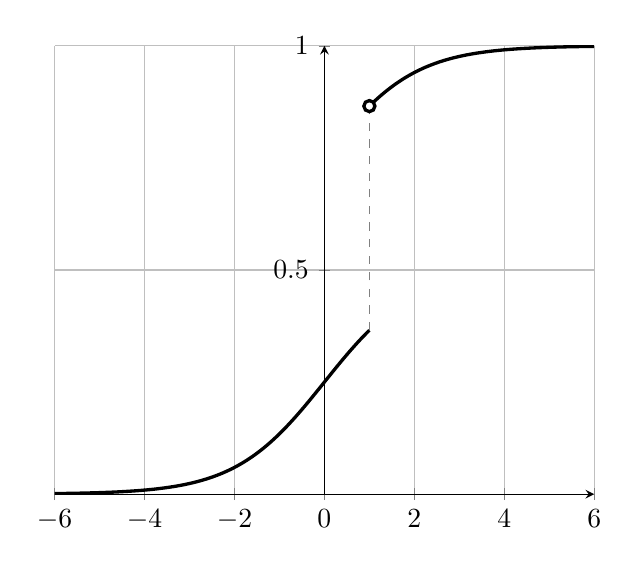
\begin{tikzpicture}[
        declare function={
            sigma(\x)=1 / (1 + exp(-\x));
            F(\x) = .5 * sigma(\x);
        }]
        \begin{axis}[
            grid=major,     
            xmin=-6, xmax=6,
            ymin=0, ymax=1,
            ytick={0,.5,1},
            axis x line=bottom,
            axis y line=middle,
            samples=100,
            legend style={at={(1,0.9)}}     
        ]
        \addplot[very thick,black,mark=none, domain=-6:1]   {F(x)};
        \addplot[very thick,black,mark=*,mark options={fill=white},domain=1:6, mark repeat=1000]    {F(x)+0.5};
        \draw [dashed,black!50] (1,{F(1)}) -- (1,{F(1)+0.5});        
        \end{axis}
    \end{tikzpicture}
\end{center}
\end{rmrk} 

\begin{defn}
    Квантили уровней, кратных $0.01$, называют \textit{процентилями}, квантили уровней, кратных $0.1$, — \textit{децилями}, уровней, кратных $0.25$, — \textit{квартилями}.
\end{defn} 

\begin{rmrk}
    Медиана является квантилем уровня $1 / 2$.
\end{rmrk} 

\begin{namedthm}[Свойства медианы]\leavevmode
\begin{enumerate}
    \item Медиана случайной величины $\xi$ минимизирует средний модуль отклонения $\xi$:
    \begin{equation*}
        \Exp |\xi - \operatorname{Med} \xi| 
    = \min _{a} \Exp |\xi-a|;
    \end{equation*}
    \item Отклонение медианы случайной величины $\xi$ от её матожидания $\Exp \xi$ не превышает по модулю среднеквадратичного отклонения $\sigma = \sqrt{\Var\xi}$:
    \begin{equation*}
        |\Exp \xi - \operatorname{Med}\xi| \leqslant \sigma.
    \end{equation*}
\end{enumerate}
\end{namedthm}

\begin{proof}
    \begin{enumerate}
        \item Рассмотрим случайную величину $\eta = \xi - \operatorname{Med}\xi$. 
        Очевидно, что $\operatorname{Med} \eta = 0$. 
        Тогда нам надо показать, что $\forall c \in \Real $ справедливо 
        \begin{equation*}
            \Exp |\eta - c| - \Exp |\eta| \geqslant 0.
        \end{equation*}
        
        Рассмотрим случай $c > 0$. Заметим, что 
        \begin{equation*}
            \begin{cases}
                |\eta - c| - |\eta| = c, & \eta < 0; \\
                |\eta - c| - |\eta|  \geqslant -c, & \eta \geqslant 0.
        \end{cases}
        \end{equation*}
        
        Тогда
        \begin{gather*}
            \Exp \bigl(|\eta - c| - |\eta| \bigl) 
            = \Exp \bigl( (|\eta - c| - |\eta|) \cdot \Ind(\eta < 0) + (|\eta - c| - |\eta|) \cdot \Ind(\eta \geqslant 0) \bigl) \\
            \Exp \bigl( |\eta - c| - |\eta| \bigl) \geqslant c~\MyPr(\eta < 0) - c~\MyPr(\eta \geqslant 0).
        \end{gather*}
        Так как $\operatorname{Med}\eta = 0$, то $\MyPr(\eta \leqslant 0) = \MyPr(\eta \geqslant 0) = \frac{1}{2} \implies \Exp \bigl( |\eta - c| - |\eta| \bigl) \geqslant 0.$.

        Случай $c < 0$ сводится к предыдущему умножением случайной величины и $c$ на $-1$. Отсюда следует, что медиана действительно минимизирует средний модуль отклонения.

        \item Рассмотрим цепочку неравенств:
        \begin{multline*}
            |\Exp \xi - \operatorname{Med}\xi| =
            |\Exp (\operatorname{Med}\xi - \xi)| \leqslant
            {\text{\{св-во (6) матожидания\}}} \leqslant 
            \Exp |\operatorname{Med}\xi - \xi| \leqslant \\ {\text{\{св-во (1) медианы\}}} \leqslant
            \Exp | \Exp \xi - \xi| = 
            \Exp \sqrt{|\Exp \xi - \xi|^2} \leqslant
            {\text{\{нер-во Йенсена\}}} \leqslant \\
            \leqslant \sqrt{\Exp | \Exp \xi - \xi|^2} = \sqrt{\Var\xi} = \sigma.
        \end{multline*}
        
    \end{enumerate}
\end{proof}
\begin{defn}
    \textit{Интерквартильным размахом} называется разность между третьим и первым квартилями, то есть ${\displaystyle x_{0{,}75}-x_{0{,}25}}.$
\end{defn} 

В каком-то смысле эту величину можно считать аналогом дисперсии случайной величины, устойчивой к выбросам.
  % Числовые характеристики случайных величин: квантили. Медиана и ее свойства. Интерквартильный размах
\section{Испытания Бернулли. Биномиальное распределение. Теорема Пуассона. Распределение Пуассона}
\begin{defn}
    \textit{Испытание Бернулли}~--- случайный эксперимент, у которого есть ровно два возможных 
    исхода: <<успех>> и <<неудача>>. 
    Как правило, вероятность успеха обозначается буквой $p$, вероятность неудачи $q = 1 - p$.
\end{defn}

\begin{defn}
    \textit{Схема Бернулли}~--- последовательность из $n$ \textit{независимых однородных} испытаний Бернулли c вероятностью успеха $p$ и неудачи $q = 1 - p$.
\end{defn}

Со схемой Бернулли можно связать последовательность случайных величин $\xi_1,\, \xi_2,\, \ldots,\, \xi_n,$ где 
$\xi_k = 
    \begin{cases} 
        1, &\text{с вероятностью } p; \\ 
        0, & \text{с вероятностью } q,
    \end{cases} 
    \quad k = \overline{1, n}$.

Таким образом, принятие случайной величиной $\xi_k$ значения $1$ интерпретируется как успех в $k$-м испытании.
Так как испытания в схеме Бернулли независимы и однородны, данные случайные величины должны быть \textit{независимы и одинаково распределены}.

\begin{namedthm}[Формула Бернулли]
    Пусть $\xi$~--- случайная величина, равная числу успехов в $n$ испытаниях. Тогда $\forall k = \overline{1,n}$ вероятность получить в $n$ испытаниях ровно $k$ успехов равна
    \begin{equation*}
        \MyPr\left(\xi=k\right)=C_{n}^{k} p^{k} q^{n-k}
    \end{equation*}
    \end{namedthm}
    
    \begin{proof}
    Рассмотрим один элементарный исход события $A = \{\xi = k \}$:
    \begin{equation*}
        (\underbrace{y, y, \ldots, y}_{k}, \underbrace{\textit{ н}, \textit{ н}, \ldots,\textit{ н}}_{n-k})
    \end{equation*}
    когда первые $k$ испытаний завершились успехом (у), остальные неудачей (н). Поскольку испытания независимы, вероятность такого элементарного исхода равна $p^k(1 - p)^{n-k}.$ Другие элементарные исходы из события $A$ отличаются лишь расположением $k$ успехов на $n$ местах. Поэтому событие $A$ состоит из $C_n^k$ элементарых исходов, вероятность каждого из которых равна $p^kq^{n-k}$.
    \end{proof}
    
    \begin{defn}
        Пусть $\xi_1, \ldots, \xi_n$~--- последовательность независимых случайных величин, имеющих одинаковое распределение Бернулли с параметром $p$ ($\Bernoulli_{p}$), то есть принимает значение $1$ (<<успех>>) с вероятностью $p$ и $0$ (<<неудача>>) с вероятностью $1 - p = q$. Тогда говорят, что случайная величина $\xi = \xi_1 + \ldots + \xi_n$ имеет \textit{биномиальное распределение} с параметрами $n$ и $p$ ($\Binom_{n, p}$).
    \end{defn}
    
    \subsubsection{Числовые характеристики $\Bernoulli_{p}$}
    \begin{enumerate}
        \item Математическое ожидание:
        \begin{equation*}
            \Exp \xi =  1 \cdot p + 0 \cdot q = p
        \end{equation*}
        \item Дисперсия:
            $$\Exp \xi^2 = 1^2 \cdot p + 0^2 \cdot q = p; \quad \Var\xi = \Exp \xi^2 - (\Exp \xi)^2 = p - p^2 = p \cdot (1 - p) = pq$$
    \end{enumerate}
    
    \subsubsection{Числовые характеристики $\Binom_{n, p}$}
    \begin{enumerate}
        \item Математическое ожидание:
        \begin{equation*}
            \Exp \xi = \Exp (\xi_1 + \ldots + \xi_n) = \Exp \xi_1 + \ldots + \Exp \xi_n = \underbrace{p + \ldots + p}_{n} = np
        \end{equation*}
        \item Дисперсия:
        \begin{equation*}
            \Var\xi = \Var(\xi_1 + \ldots + \xi_n) = \Var\xi_1 + \ldots + \Var\xi_n = \underbrace{p \cdot q + \ldots + p \cdot q}_{n} = npq
        \end{equation*}
    \end{enumerate}
    
    \begin{namedthm}[Теорема Пуассона]
        Пусть проводится $n$ обобщённых испытаний Бернулли (т.е. вероятность успеха испытания зависит от $n$) с вероятностью успеха $p_n$, $\xi$~--- количество успехов в этих испытаниях и $n p_{n} \underset{n \to +\infty}{\longrightarrow} \lambda$. Тогда
        \begin{equation*}
            \forall k \in \Integer,~ 0 \leqslant k \leqslant n: \quad \MyPr\left(\xi=k\right) \underset{n \to +\infty}{\longrightarrow} \frac{\lambda^{k}}{k !} e^{-\lambda}
        \end{equation*}
    \end{namedthm}
    
    \begin{proof}
        По условию теоремы, $n p_n \xrightarrow[n \to +\infty]{} \lambda$. Тогда $p_n \xrightarrow[n \to +\infty]{} 0$. Рассмотрим формулу Бернулли:
        \begin{multline*}
            \MyPr(\xi = k) = C_n^k p^k (1 - p)^{n-k} = \frac{n!}{k!(n - k)!} \cdot \frac{\lambda^k}{n^k} \cdot \left(1 - \frac{\lambda}{n}\right)^{-k} \cdot \left(1 - \frac{\lambda}{n}\right)^n = \\
            = \frac{\lambda^k}{k!} \cdot \frac{(n - k + 1) \cdot \ldots \cdot (n - 1) \cdot n}{n^k} \cdot \left(1 - \frac{\lambda}{n}\right)^n \cdot \left(1 - \frac{\lambda}{n}\right)^{-k}
        \end{multline*}
        Перейдём к пределу при $n \to +\infty$:
        \begin{equation*}
            \frac{(n - k + 1) \cdot \ldots \cdot (n - 1) \cdot n}{n^k} \to 1,~ \left(1 - \frac{\lambda}{n}\right)^n \to e^{-\lambda},~ \left(1 - \frac{\lambda}{n}\right)^{-k} \to 1
        \end{equation*}
        
        Таким образом, получим
        \begin{equation*}
            \MyPr(\xi = k) \xrightarrow[n \to +\infty]{} \frac{\lambda^k}{k!} e^{-\lambda}
        \end{equation*}
    \end{proof}
    
    \begin{defn}
        Набор вероятностей $\{\frac{\lambda^k}{k!} e^{-\lambda} \}$, где $k$ принимает значения $0, 1, 2, \ldots$, называется \textit{распределением Пуассона} с параметром $\lambda > 0$ ($\Pois_{\lambda}$).
    \end{defn}
    \begin{rmrk}
        Распределение Пуассона представляет собой число событий, произошедших за фиксированное время, при условии, что данные события происходят с некоторой фиксированной средней интенсивностью (за которую отвечает параметр $\lambda$) и независимо друг от друга.
    \end{rmrk}
    
    \subsubsection{Числовые характеристики $\Pois_{\lambda}$}
    \begin{enumerate}
        \item Математическое ожидание:
        \begin{align*}
            \sum\limits_{k=0}^{\infty} e^{-\lambda} \frac{\lambda^k}{k!} = e^{-\lambda} \sum\limits_{k=0}^{\infty} \frac{\lambda^k}{k!} = e^{-\lambda} e^\lambda = 1 \\
            \Exp \xi = \sum\limits_{k=1}^{\infty} k e^{-\lambda} \frac{\lambda^k}{k!} = e^{-\lambda} \lambda \underbrace{\sum\limits_{k=1}^{\infty} \frac{\lambda^{k-1}}{(k - 1)!}}_{= e^\lambda} = \lambda
        \end{align*}
        \item Дисперсия:
        \begin{align*}
            \Exp \xi(\xi - 1) = \sum\limits_{k=0}^{\infty} k (k - 1) \frac{\lambda^k}{k!} e^{-\lambda}  = \lambda^2 e^{-\lambda} \sum\limits_{k=2}^{\infty} \frac{\lambda^{k-2}}{(k-2)!} = \lambda^2 e^{-\lambda} e^\lambda = \lambda^2 \\
            \Exp \xi^2 = \Exp \xi(\xi - 1) + \Exp \xi = \lambda^2 + \lambda \quad \implies \quad \Var\xi = \Exp \xi^2 - (\Exp \xi)^2 = \lambda
        \end{align*}
    \end{enumerate}  % Испытания Бернулли. Биномиальное распределение. Теорема Пуассона. Распределение Пуассона
\section{Испытания Бернулли. Геометрическое распределение. Теорема Реньи. Показательное распределение}
Рассмотрим бесконечную схему экспериментов Бернулли с вероятностью успеха $p$, неудачи~--- $q = 1 - p$. 
Вероятность того, что первый успех произойдёт в испытании с номером $k \in \Natural$, очевидно, равна $\MyPr(\tau = k) = pq^{k-1}$.
Действительно, это событие равносильно тому, что $\xi_1 = \xi_2 = \ldots = \xi_{k-1} = 0,\: \xi_k = 1$. 
В силу независимости~$\xi_i$
\begin{multline*}
    \MyPr(\xi_1 = 0,\, \xi_2 = 0, \ldots, \xi_{k-1} = 0,\, \xi_k = 1) = \\
    \MyPr(\xi_1 = 0) \cdot \MyPr(\xi_2 = 0) \cdot \ldots \cdot \MyPr(\xi_{k-1} = 0) \cdot \MyPr(\xi_k = 1) =
    q^{k-1}p.
\end{multline*}

\begin{defn}
    Набор вероятностей $\{p q^{k-1}\}$, где $k$ принимает любые значения из множества натуральных чисел, называется \textit{геометрическим распределением} вероятностей ($\Geom_{p}$).
\end{defn}

Аналогично можно ввести геометрическое распределение как <<число неудач до первого успеха>>. 
Тогда $k$ будет принимать значения из множества $\{0, 1, 2, \ldots\}$, и $\MyPr(\tau^{\prime} = k) = pq^k$.

\subsubsection{Числовые характеристики $\Geom_{p}$}
\begin{enumerate}
    \item Математическое ожидание:
    \begin{multline*}
        \Exp \xi=\sum\limits_{k=1}^{\infty} k p q^{k-1}=p \sum\limits_{k=1}^{\infty} k q^{k-1}=p \sum\limits_{k=1}^{\infty} \frac{d q^{k}}{d q} = \\
        = p \frac{d}{d q}\left(\sum\limits_{k=1}^{\infty} q^{k}\right)=p \frac{d}{d q}\left(\frac{q}{1-q}\right)=p \frac{1}{(1-q)^{2}}=\frac{1}{p}.
    \end{multline*}
    \item Дисперсия:
    \begin{multline*}
        \Exp \xi(\xi-1)=\sum\limits_{k=1}^{\infty} k(k-1) p q^{k-1}=p q \sum\limits_{k=0}^{\infty} \frac{d^{2} q^{k}}{d q^{2}} =p q \frac{d^{2}}{d q^{2}}\left(\sum\limits_{k=0}^{\infty} q^{k}\right) = \\
        =p q \frac{d^{2}}{d q^{2}}\left(\frac{1}{1-q}\right)=p q \frac{2}{(1-q)^{3}}=\frac{2 q}{p^{2}} \\
        \Var \xi=\Exp \xi(\xi-1)+\Exp \xi-(\Exp \xi)^{2}=\frac{2 q}{p^{2}}+\frac{1}{p}-\frac{1}{p^{2}}=\frac{2 q-1+p}{p^{2}}=\frac{q}{p^{2}}.
    \end{multline*}
\end{enumerate}

\begin{rmrk}
    Если определять геометрическое распределение как количество неудач до первого успеха, его математическое ожидание изменится:
    \begin{multline*}
        \Exp \xi=\sum\limits^{\infty}_{\color{red}k=0} k p q^{\color{red}k}= {\color{red}q}p \sum\limits_{k=1}^{\infty} k q^{k-1}= {\color{red}q}p \sum\limits_{k=1}^{\infty} \frac{d q^{k}}{d q} = \\
        = {\color{red}q}p \frac{d}{d q}\left(\sum\limits_{k=1}^{\infty} q^{k}\right)={\color{red}q} p \frac{d}{d q}\left(\frac{q}{1-q}\right)= {\color{red}q}p \frac{1}{(1-q)^{2}}=\frac{{\color{red}q}}{p}
    \end{multline*}
    Так как $q \in (0,1)$, математическое ожидание станет меньше, и это логично~--- ведь количество неудач до первого успеха всегда на единицу меньше номера первого успеха. 
    (Используя это наблюдение, можно посчитать матожидание ещё проще~--- $\Exp (\xi - 1) = \frac{1}{p} - 1 = \frac{1-p}{p} = \frac{q}{p}$). 
    Дисперсия же не зависит от сдвига и останется прежней.
\end{rmrk}

\begin{defn}
    Случайная величина $\xi$ имеет \textit{показательное (экспоненциальное) распределение} с параметром $\lambda > 0$ ($\ExpDist_{\lambda}$), 
    если $\xi$ имеет следующие плотность и функцию распределения:
    \begin{equation*}
        f(x) = 
        \begin{cases}
            0, & \text{если $x < 0$;} \\
            \lambda e^{-\lambda x}, & \text{если $x \geqslant 0$.}
        \end{cases}
        \quad 
        F(x) = 
        \begin{cases}
            0, & \text{если $x < 0$;} \\
            1 - e^{-\lambda x}, & \text{если $x \geqslant 0$.}
        \end{cases}
    \end{equation*}
\end{defn}

\begin{rmrk}
    Показательное распределение моделирует время между двумя последовательными свершениями одного и того же события. 
    К примеру, пусть есть магазин, в который время от времени заходят покупатели. 
    При определённых допущениях время между появлениями двух последовательных покупателей будет случайной величиной с экспоненциальным распределением. 
    Среднее время ожидания нового покупателя равно $\frac{1}{\lambda}$. 
    Сам параметр $\lambda$ тогда может быть интерпретирован как среднее число новых покупателей за единицу времени. 
\end{rmrk}

\subsubsection{Числовые характеристики $\ExpDist_{\lambda}$}

Найдём для произвольного $k \in \Natural$ момент порядка $k$:
\begin{equation*}
    \Exp \xi^{k}=\int\limits_{-\infty}^{\infty} x^{k} f_{\xi}(x) d x=\int\limits_{0}^{\infty} x^{k} \lambda e^{-\lambda x} d x=\frac{1}{\lambda^{k}} \int\limits_{0}^{\infty}(\lambda x)^{k} e^{-\lambda x} d(\lambda x)=\frac{k !}{\lambda^{k}}
\end{equation*}

В последнем равенстве была использована формула для гамма-функции:
\begin{equation*}
    \Gamma(k+1)=\int\limits_{0}^{\infty} u^{k} e^{-u} d u=k !
\end{equation*}
\begin{enumerate}
    \item Математическое ожидание: $\Exp \xi=\frac{1}{\lambda}$.
    \item Дисперсия: $\Exp \xi^{2}=\frac{2}{\lambda^{2}}, ~ \Var \xi=\Exp \xi^{2}-(\Exp \xi)^{2}=\frac{1}{\lambda^{2}}$.
\end{enumerate}

Важным требованием в схеме Бернулли является однородность, т.е. постоянство параметра $p$ на протяжении всех испытаний.
Но иногда есть желание посмотреть, например, что получится, если устремить вероятность успеха к нулю, а количество испытаний к бесконечности. В этом случае придётся прибегнуть к нетривиальной модели эксперимента.
\begin{thm*}
    Рассмотрим серию схем Бернулли~--- последовательность схем Бернулли с количеством испытаний $n$ и вероятностями успеха $p_n$ (т.е. в первой схеме~--- одно испытание с вероятностью успеха $p_1$, в второй~--- два испытания с вероятностью успеха $p_2$ и т.д.). В каждой схеме рассмотрим случайную величину $\tau_n \sim \Geom_{p_n}$.
    Пусть $n p_n \xrightarrow[n \to \infty]{} \lambda > 0$.

    Тогда распределение случайной величины $\frac{\tau_n}{n}$ сходится к показательному с параметром $\lambda$ при $n \to +\infty$.
\end{thm*}

\begin{proof}
    Пусть $F_n$~--- функция распределения случайной величины $\frac{\tau_n}{n}$.
    Тогда для $x \geqslant 0$:
    \begin{multline*}        
        F_{n}(x)=\MyPr\left(\frac{\tau_{n}}{n} \leqslant x\right)=
        \MyPr\left(\tau_{n} \leqslant n x\right) = 
        \MyPr\left(\tau_{n} \leqslant \lfloor n x\rfloor\right) = \\
        = \sum\limits_{k = 1}^{\lfloor nx \rfloor} p_n q_n^{k-1} = 
        p_n \, \frac{1 - q_n^{\lfloor nx \rfloor + 1}} {1-q_n} = 
        1-\left(1-p_{n}\right)^{\lfloor nx \rfloor + 1}
    \end{multline*}
    
    Далее, т.к. $\left(1-p_{n}\right)^{n}=\left(1-\frac{n p_{n}}{n}\right)^{n} \xrightarrow[n \to +\infty]{} e^{-\lambda}$, 
    то $(1 - p_n)^{nx} \xrightarrow[n \to +\infty]{} e^{-\lambda x}.$ 
    По определению, $\lfloor n x\rfloor \leqslant n x<\lfloor n x\rfloor\,+\,1$, 
    или, что эквивалентно, $nx < \lfloor nx \rfloor \,+\,1 \leqslant nx\,+\,1$. 
    Таким образом верно $(1 - p_n)^{\lfloor nx \rfloor + 1} \xrightarrow[n \to +\infty]{} e^{-\lambda x}$. 
    Следовательно, $F_n(x) \xrightarrow[n \to +\infty]{} 1 - e^{-\lambda x}$, что есть функция показательного распределения. 
\end{proof}

%sec1-8
\begin{center}
    \begin{tikzpicture}[
        declare function={
            exp_pdf(\x,\l) = \l * exp(-\l*  \x);
            geom_pmf(\x,\p) = \p * (1 - \p)^(\x);
        }]
        \begin{axis}[
            height=9cm, width=18cm,
            xmin=0, xmax=6,
            ymin=0, ymax=0.6,
            xlabel={$x$},
            ylabel={$f(x)$},
            xtick={0.5, 1, ..., 5.5},
            ytick={0.1, 0.2, ..., 0.5},
            axis line style=thick,
            axis lines=middle,
            enlargelimits=false
            ]
            \addplot[very thick, black, domain=0:5.5] {exp_pdf(x,0.5)};
            \addplot[color=red, domain=0:5, samples=6, mark=*] {geom_pmf(x,0.5)};
            \legend{$\ExpDist_{0.5}$, $Geom_{0.5}$}
        \end{axis}
    \end{tikzpicture}
\end{center}

\begin{namedthm}[Теорема Реньи]
Пусть даны случайная величина $N \sim \Geom_{p}$, $\xi_1, \xi_2, \ldots$~--- независимые одинаково распределённые случайные величины, 
$\xi_i \geqslant 0$ и $0 < a = \Exp \xi_i < \infty$, $S_n = \sum\limits_{i=1}^N \xi_i$. Тогда
\begin{equation*}
    \sup\limits_{x}\left|\MyPr\left(\frac{p}{a} S_{N}<x\right)-G(x)\right| \underset{p \to 0}{\longrightarrow} 0,
\end{equation*}

где $G(x)=\left(1-e^{-x}\right) \Ind(x \geqslant 0)$~--- функция стандартного показательного распределения $\ExpDist_{1}$.

Если $b^2 = \Exp \xi_i^2$, то $\sup\limits_{x}\left|\MyPr\left(\frac{p}{a} S_{N}<x\right)-G(x)\right| \leqslant \frac{p b^{2}}{(1-p) a^{2}}$.
\end{namedthm}
  % Испытания Бернулли. Геометрическое распределение. Теорема Реньи. Показательное распределение
\section{Испытания Бернулли. Теорема Муавра"--~Лапласа. Нормальное распределение}

\begin{namedthm} [Локальная предельная теорема Муавра"--~Лапласа]
    Пусть $S_n$~--- число успехов в $n$ испытаниях Бернулли с вероятностью успеха $0 < p < 1$. 
    Пусть $n \to \infty$, тогда $n p(1-p) {\longrightarrow} \infty$, и 
    \begin{equation*}
        \forall m \in \Integer: 0 \leqslant m \leqslant n \quad \MyPr\left(S_{n}=m\right)=\frac{1}{\sigma \sqrt{2 \pi} } e^{-\frac{x^{2}}{2}}\left(1+\underline{O}\left(\frac{1}{\sigma}\right)\right),
    \end{equation*}
    где $x = \frac{m - np}{\sigma},$ а $\sigma=\sqrt{\Var S_{n}}=\sqrt{n p(1-p)}$.
\end{namedthm}  

\begin{namedthm}[Интегральная теорема Муавра"--~Лапласа]
    Пусть $S_n$~--- число успехов в $n$ испытаниях Бернулли с вероятностью успеха $0 < p < 1$, $C$~--- произвольная положительная константа, тогда равномерно по $a$ и $b$ из отрезка $[-C,C]$ (пусть $b \geqslant a$)
\begin{equation*}
    \MyPr\left(a \leqslant \frac{S_{n}-n p}{\sqrt{n p(1-p)}} \leqslant b\right) \xrightarrow[n \to +\infty]{} \frac{1}{\sqrt{2 \pi}} \int\limits_{a}^{b} e^{-\frac{x^{2}}{2}} dx.
\end{equation*}
\end{namedthm} 

\begin{defn}
    Случайная величина $\xi$ имеет \textit{нормальное (гауссовское) распределение} с параметрами $a$ и $\sigma^2$ ($\Normal_{a, \sigma^2}$), где $a \in \Real, \sigma > 0$, если $\xi$ имеет следующую плотность распределения: 
\begin{equation*}
    f(x)=\frac{1}{\sigma \sqrt{2 \pi}} e^{-\frac{(x-a)^{2}}{2 \sigma^{2}}}, \quad x \in \Real.
\end{equation*}
\end{defn}

\subsubsection{Числовые характеристики $\Normal_{a, \sigma^2}$}

Найдем матожидание и дисперсию для \textit{стандартного} нормального распределения ($\alpha = 0, \, \sigma^2 = 1$):
\begin{multline*}
    \Exp \xi = 
    \int\limits_{-\infty}^{\infty} x f_{\xi}(x) dx =
    \frac{1}{\sqrt{2\pi}} \int\limits_{-\infty}^{\infty} x e^{\frac{-x^2}{2}} dx = 
    -\frac{1}{\sqrt{2\pi}} \int\limits_{-\infty}^{\infty} d\left( e^{\frac{-x^2}{2}}\right) = 
    \left. -e^{\frac{-x^2}{2}}\right|_{-\infty}^{\infty} = 0 \\
    \Exp \xi^{2}=\frac{1}{\sqrt{2 \pi}} \int\limits_{-\infty}^{\infty} x^{2} e^{-x^{2} / 2} d x=\frac{2}{\sqrt{2 \pi}} \int\limits_{0}^{\infty} x^{2} e^{-x^{2} / 2} d x=-\frac{2}{\sqrt{2 \pi}} \int\limits_{0}^{\infty} x d e^{-x^{2} / 2}= \\
    =-\left.\frac{2 x}{\sqrt{2 \pi}} e^{-x^{2} / 2}\right|_{0} ^{\infty}+2 \int\limits_{0}^{\infty} \frac{1}{\sqrt{2 \pi}} e^{-x^{2} / 2} d x=0+\int\limits_{-\infty}^{\infty} \frac{1}{\sqrt{2 \pi}} e^{-x^{2} / 2} d x=1.
\end{multline*}

Поэтому $\Var\xi = \Exp \xi^2 - (\Exp \xi)^2 = 1 - 0 = 1.$

Теперь рассмотрим случайную величину $\eta$ с нормальным распределением в общем виде (с параметрами $\alpha$ и $\sigma^2$). Тогда $\xi = \frac{\eta - \alpha}{\sigma}$ - случайная величина со \textit{стандартным} нормальным распределением. Далее, т.к. $\Exp \xi = 0$, $\Var\xi = 1$, то 
\begin{gather*}
    \Exp \eta = \Exp (\sigma \xi + \alpha) = \sigma \Exp \xi + \alpha = \alpha, \\
    \Var\eta = \Var(\sigma \xi + \alpha) = \sigma^2 \Var\xi = \sigma^2.
\end{gather*}
%sec1-9
\begin{center}
    \begin{tikzpicture}[
        declare function={
            normal_pdf(\x,\sstd,\mu) = 1 / sqrt(2 * pi * \sstd) * exp(-(\x - \mu)^2 / (2 * \sstd));
            binom_pmf(\x,\n,\p) = \n! / (\x! * (\n - \x)!) * \p^(\x) * (1 - \p)^(\n - \x);
            pois_pmf(\x,\l) = \l^(\x) * exp(-\l) / (\x!);
        }]
        \begin{axis}[
            height=11cm, width=18cm,
            xmin=0, xmax=11,
            ymin=-0.05, ymax=0.45,
            xlabel={$x$},
            ylabel={$f(x)$},
            xtick={1, ..., 10},
            ytick={0.1, 0.2, ..., 0.4},
            axis line style=thick,
            axis lines=middle,
            enlargelimits=false
            ]
            \addplot[very thick, color1, samples=100,domain=0:10] {normal_pdf(x,2.5,5)};
            \addplot[color=red, domain=0:10, samples=11, mark=*] {binom_pmf(x,10,0.5)};
            \addplot[color=color2, domain=0:10, samples=11, mark=*] {pois_pmf(x,1)};
            \addplot[color=blue, domain=0:10, samples=11, mark=*] {pois_pmf(x,3)};
            \addplot[color=black, domain=0:10, samples=11, mark=*] {pois_pmf(x,5)};
            \legend{$\Normal_{5;2.5}$, $\Binom_{10;0.5}$, $\Pois_{1}$, $\Pois_{3}$, $\Pois_{5}$}
        \end{axis}
    \end{tikzpicture}
\end{center}
\vspace{1cm}
\begin{rmrk}
Формулу из теоремы Муавра"--~Лапласа можно переписать в следующем виде:
\begin{equation*}
    \MyPr\left(a \leqslant \frac{S_{n}-n p}{\sqrt{n p(1-p)}} \leqslant b\right) \xrightarrow[n \to +\infty]{} \Phi(b) - \Phi(a),
\end{equation*}
где $\Phi(x)=\frac{1}{\sqrt{2 \pi}} \int\limits_{-\infty}^{x} e^{-t^{2} / 2} d t$~--- функция распределения стандартного нормального распределения.
\end{rmrk}  % Испытания Бернулли. Теорема Муавра—Лапласа. Нормальное распределение
\section{Совокупности случайных величин. Совместная функция распределения. Независимость случайных величин. Критерии независимости. Ковариация, коэффициент корреляции}

\subsubsection{Совместное распределение, его свойства}

Пусть случайные величины $\xi_1, \ldots, \xi_n$ заданы на одном вероятностном пространстве $(\Omega, \SigAlg \MyPr)$.
\begin{defn}
    \textit{Совместное распределение} случайных величин $(\xi_1, \ldots, \xi_n)$~--- функция $\MyPr\colon \Borel(\Real^{n}) \to \Real$:
    \begin{equation*}
        \MyPr(\xi \in B) = \MyPr(\omega \colon (\xi_{1}(\omega), \ldots, \xi_{n}(\omega)) \in B),~ B \subset \Borel(\Real^{n}).
    \end{equation*}
\end{defn}
\begin{defn}
    \textit{Функция совместного распределения} случайных величин $(\xi_1, \ldots, \xi_n)$~--- функция $F\colon \Real^{n} \to \Real$:
    \begin{equation*}
        F(x_{1}, \ldots, x_{n})=\MyPr(\xi_{1}<x_{1}, \ldots, \xi_{n}<x_{n}).
    \end{equation*}
\end{defn}

\begin{rmrk}
    Для функции совместного распределения выполняются свойства, аналогичные одномерному случаю~--- сохраняется монотонность, непререрывность слева по каждой переменной.
    При этом частные функции распределения восстанавливаются по совместной следующим образом:
    \begin{equation*}
        \lim\limits_{\substack{x_{k} \to +\infty \\ k \neq i}}  F(x_{1}, \ldots, x_{i}, \ldots, x_{n}) = F_{i}(x), \quad i = \overline{1,n}.
    \end{equation*}
    Следует, однако, обратить внимание на предельные свойства. 
    Для простоты проиллюстрируем их на двумерном случае.
    \begin{align*}
        \lim\limits_{x_1 \to -\infty} F(x_1, x_2) & = 0 \\
        \lim\limits_{x_2 \to -\infty} F(x_1, x_2) & = 0 \\
        \lim_{
            \substack{
                x_1 \to +\infty \\ 
                x_2 \to +\infty
            }
        } F(x_1, x_2) & = 1
    \end{align*}
    В самом деле, по определению $F(x_1, x_2) = \MyPr(\xi_1 < x_1, \xi_2 < 2) = \MyPr(B_1 \cap B_2),$ 
    где $B_1 = \{\xi_1 < x_1\}, B_2 = \{\xi_2 < x_2\}$. 
    Если хоть одно из событий "<стремится"> к пустому множеству (что и происходит при $x_1 \to -\infty$ или $x_2 \to -\infty$), 
    то и пересечение делает то же самое.

    Если же мы хотим получить в пересечении $\Omega$ (и, следовательно, вероятность~$1$), то необходимо устремить $x_1$ и $x_2$ к $+\infty$ \textit{одновременно}.
\end{rmrk}

Далее рассматриваем совместные распределения двух случайных величин.

\subsubsection{Виды многомерных распределений}

\begin{defn}
    Случайные величины $\xi_1, \xi_2$ имеют дискретное совместное распределение, если существует не более чем счётный набор пар неотрицательных чисел $\{a_{i}, b_{j}\}$ такой, что
    \begin{equation*}
        \sum\limits_{i=1}^{\infty} \sum\limits_{j=1}^{\infty} \MyPr\left(\xi_{1}=a_{i}, \xi_{2}=b_{j}\right)=1.
    \end{equation*}
    Таблицу, на пересечении $i$-й строки и $j$-го столбца которой стоит вероятность $\MyPr\left(\xi_{1}=a_{i}, \xi_{2}=b_{j}\right)$, называют \textit{таблицей совместного распределения} случайных величин $\xi_1$ и $\xi_2$.
\end{defn}
\begin{defn}
    Случайные величины $\xi_1, \xi_2$ имеют абсолютно непрерывное совместное распределение, если существует неотрицательная функция $f_{\xi_{1}, \xi_{2}}(x, y)$ такая, что для любого борелевского множества $B \in \Borel\left(\Real^{2}\right)$ имеет место равенство
    \begin{equation*}
        \MyPr\bigl(\left(\xi_{1}, \xi_{2}\right) \in B\bigr)=\iint\limits_{B} f_{\xi_{1}, \xi_{2}}(x, y) \, dx dy.
    \end{equation*}
    Если такая функция $f_{\xi_{1}, \xi_{2}}(x, y)$ существует, она называется \textit{плотностью совместного распределения} случайных величин $\xi_1, \xi_2$.
    
    Функция совместного распределения в этом случае имеет вид:
    \begin{equation*}
        F(x, y)=\MyPr(\xi_{1}<x, \xi_{2}<y)=\int\limits_{-\infty}^{x}\left(\int\limits_{-\infty}^{y} f_{\xi_{1}, \xi_{2}}(u, v) \, dv\right) du.
    \end{equation*}
\end{defn}

\begin{rmrk}
    Плотность совместного распределения имеет те же свойства, что и плотность распределения одной случайной величины: неотрицательность и нормированность:
    \begin{equation*}
        f(x, y) \geqslant 0~ \forall x, y \in \Real, \quad \iint\limits_{\Real^{2}} f(x, y) \, dx dy = 1.
    \end{equation*}

    По функции совместного распределения его плотность находится как смешанная частная производная (в точках, где она существует):
    \begin{equation*}
        f(x, y)=\frac{\partial^{2}}{\partial x \partial y} F(x, y).
    \end{equation*}
\end{rmrk}

\begin{rmrk}
    Из существования плотностей $\xi_1$ и $\xi_2$ не следует абсолютная непрерывность совместного распределения этих случайных величин. 
    Например, вектор $(\xi, \xi)$ принимает значения только на диагонали в $\Real^2$ и уже поэтому не имеет плотности распределения (его распределение сингулярно). 
    Обратное же свойство, как показывает следующая теорема, всегда верно.
\end{rmrk}

\begin{thm*}
    Если случайные величины $\xi_1$ и $\xi_2$ имеют абсолютно непрерывное совместное распределение с плотностью $f(x, y)$, то $\xi_1$ и $\xi_2$ в отдельности также имеют абсолютно непрерывное распределение с плотностями:
    \begin{equation*}
        f_{\xi_{1}}(x)=\int\limits_{-\infty}^{\infty} f(x, y) dy, \quad f_{\xi_{2}}(y)=\int\limits_{-\infty}^{\infty} f(x, y) dx.
    \end{equation*}
    Для $n > 2$ плотности случайных величин $\xi_1, \ldots, \xi_n$ находятся по плотности их совместного распределения $f(x_1, \ldots, x_n)$ интегрированием функции $f$ по всем <<лишним>> координатам.
\end{thm*}
\begin{proof}
\begin{equation*}
    F_{\xi_{1}}\left(x_{1}\right)
    = \lim _{x_{2} \to+\infty} F_{\xi_{1}, \xi_{2}}\left(x_{1}, x_{2}\right)
    = \int\limits_{-\infty}^{x_{1}}\left(\int\limits_{-\infty}^{\infty} f(x, y) d y\right) d x
    = \int\limits_{-\infty}^{x_{1}} f_{\xi_{1}}(x) d x
\end{equation*}
\end{proof}

\subsubsection{Независимость случайных величин}
\begin{defn}
    Случайные величины $\xi_1, \ldots, \xi_n$ называют \textit{независимыми в совокупности}, если для любого набора борелевских множеств $B_{1}, \ldots, B_{n} \in \Borel(\Real)$:
    \begin{equation*}
        \MyPr\left(\xi_{1} \in B_{1}, \ldots, \xi_{n} \in B_{n}\right)=\MyPr\left(\xi_{1} \in B_{1}\right) \cdot \ldots \cdot \MyPr\left(\xi_{n} \in B_{n}\right)
    \end{equation*}
\end{defn}
\begin{namedthm}[Критерий независимости]
    Случайные величины $\xi_1, \ldots, \xi_n$ независимы в совокупности $\iff$ имеет место равенство:
    \begin{equation*}
        F_{\xi_{1}, \ldots, \xi_{n}}\left(x_{1}, \ldots, x_{n}\right)=F_{\xi_{1}}\left(x_{1}\right) \cdot \ldots \cdot F_{\xi_{n}}\left(x_{n}\right).
    \end{equation*}
    В частности, в случае дискретного совместного распределения:
    \begin{equation*}
        \MyPr\left(\xi_{1}=a_{1}, \ldots, \xi_{n}=a_{n}\right)=\MyPr\left(\xi_{1}=a_{1}\right) \cdot \ldots \cdot \MyPr\left(\xi_{n}=a_{n}\right) \quad \forall a_1, \ldots, a_n \in \Real.
    \end{equation*}
    В случае абсолютно непрерывного:
    \begin{equation*}
        f_{\xi_{1}, \ldots, \xi_{n}}\left(x_{1}, \ldots, x_{n}\right)=f_{\xi_{1}}\left(x_{1}\right) \cdot \ldots \cdot f_{\xi_{n}}\left(x_{n}\right).
    \end{equation*}
\end{namedthm}

\subsubsection{Формула свёртки}
Пусть $\xi_1, \xi_2$~--- случайные величины с плотностью совместного распределения $f_{\xi_{1}, \xi_{2}}\left(x_{1}, x_{2}\right)$, задана борелевская функция $g\colon \Real^{2} \to \Real$. 
Требуется найти функцию распределения (и плотность, если она существует) случайной величины $\eta=g\left(\xi_{1}, \xi_{2}\right)$.
\begin{lem}
    Пусть $x \in \Real$, задана область $D_{x} \subseteq \Real^{2},~ D_x = \{(u,v)\colon g(u,v) < x\}$ Тогда случайная величина $\eta=g\left(\xi_{1}, \xi_{2}\right)$ имеет функцию распределения
    \begin{equation*}
        F_{\eta}(x)=\MyPr\left(g\left(\xi_{1}, \xi_{2}\right)<x\right)=\MyPr\left(\left(\xi_{1}, \xi_{2}\right) \in D_{x}\right)=\iint\limits_{D_{x}} f_{\xi_{1}, \xi_{2}}(u, v) du dv.
    \end{equation*}
\end{lem}
Далее считаем, что случайные величины $\xi_1$ и $\xi_2$ независимы, т. е. $f_{\xi_{1}, \xi_{2}}(u, v) \equiv f_{\xi_{1}}(u) f_{\xi_{2}}(v)$. В этом случае распределение величины $g\left(\xi_{1}, \xi_{2}\right)$ полностью определяется частными распределениями величин $\xi_1$ и $\xi_2$.
\begin{namedthm}[Формула свёртки]
    Если случайные величины $\xi_1$ и $\xi_2$ независимы и имеют абсолютно непрерывные распределения с плотностями $f_{\xi_{1}}(u)$ и $f_{\xi_{2}}(v)$, то плотность распределения суммы $\xi_{1}+\xi_{2}$ существует и равна <<свёртке>> плотностей $f_{\xi_{1}}$ и $f_{\xi_{2}}$:
    \begin{equation*}
        f_{\xi_{1}+\xi_{2}}(t)=\int\limits_{-\infty}^{\infty} f_{\xi_{1}}(u) f_{\xi_{2}}(t-u) du=\int\limits_{-\infty}^{\infty} f_{\xi_{2}}(u) f_{\xi_{1}}(t-u) du.
    \end{equation*}
\end{namedthm}

\begin{proof}
    Воспользуемся утверждением вышеуказанной леммы для борелевской функции $g(u, v)=u+v$. 
    Интегрирование по двумерной области $D_{x}=\{(u, v) \colon u+v<x\}$ можно заменить последовательным вычислением двух интегралов: 
    наружного — по переменной $u$, меняющейся в пределах от $-\infty$ до $+\infty$, и внутреннего~--- по переменной $v$, которая при каждом $u$ должна быть меньше, чем $x-u$. 
    Поэтому
    \begin{equation*}
        F_{\xi_{1}+\xi_{2}}(x)=\iint\limits_{D_{x}} f_{\xi_{1}}(u) f_{\xi_{2}}(v) dv du=\int\limits_{-\infty}^{\infty}\left(\int\limits_{-\infty}^{x-u} f_{\xi_{1}}(u) f_{\xi_{2}}(v) dv\right) du.
    \end{equation*}
    
    Сделаем в последнем интеграле замену $v=t-u$. При этом $v \in(-\infty, x-u) \iff t \in(-\infty, x), d v=d t$. 
    В полученном интеграле меняем порядок интегрирования:
    \begin{equation*}
        F_{\xi_{1}+\xi_{2}}(x)=\int\limits_{-\infty}^{\infty} \int\limits_{-\infty}^{x} f_{\xi_{1}}(u) f_{\xi_{2}}(t-u) d t d u=\int\limits_{-\infty}^{x}\left(\int\limits_{-\infty}^{\infty} f_{\xi_{1}}(u) f_{\xi_{2}}(t-u) du\right) dt.
    \end{equation*}
    Из функции распределения $F_{\xi_{1}+\xi_{2}}(x)$ выражается плотность $f_{\xi_{1}+\xi_{2}}(t)$.
\end{proof}

\subsubsection{Ковариация, коэффициент корреляции, их свойства}

\begin{defn} Рассмотрим случайные величины $\xi$ и $\eta$. 
Дисперсия их суммы в общем случае равна $\Var(\xi+n)=\Var \xi+\Var \eta + 2 \bigl( \Exp (\xi \eta)-\Exp \xi \, \Exp \eta \bigr)$. Величина $\operatorname{cov}(\xi, \eta) \equiv \Exp (\xi \eta)-\Exp \xi \, \Exp \eta$ называется \textit{ковариацией} случайных величин $\xi$ и $\eta$. Если $\xi$ и $\eta$ независимы, то $\operatorname{cov}(\xi, \eta) = 0$. Обратное, вообще говоря, неверно.
\end{defn}

\hypertarget{counter_exmp_independence}{}
\begin{exmp}
    Рассмотрим $\xi \sim \Uniform_{[-\pi;\pi]}$, случайные величины ${\eta_{1}=\cos \xi}$ и ${\eta_{2}=\sin \xi}$.
    \begin{enumerate}
        \item 
            Докажем некореллированность данных случайных величин.
            \begin{gather*}
                \Exp \eta_{1}=\int\limits_{-\pi}^{\pi} \cos x \cdot \frac{1}{2 \pi} d x=0, \quad \Exp \eta_{2}=\int\limits_{-\pi}^{\pi} \sin x \cdot \frac{1}{2 \pi} d x=0 \\
                \Exp \eta_{1} \eta_{2}=\int\limits_{-\pi}^{\pi}(\cos x \sin x) \frac{1}{2 \pi} d x=\frac{1}{4 \pi} \int\limits_{-\pi}^{\pi} \sin 2 x d x=0
            \end{gather*}
            Следовательно, $\operatorname{cov}(\eta_1, \eta_2) = 0$.
        \item 
            Докажем зависимость $\eta_1$ и $\eta_2$. Рассмотрим события:
            \begin{equation*}
                A = \left\{\omega \colon \eta_1(\omega) \in \left[0, \frac{1}{2} \right] \right\}, \quad
                B = \left\{\omega \colon \eta_2(\omega) \in \left[0, \frac{1}{2} \right] \right\},
            \end{equation*}
            Проверим по критерию независимости:
            \begin{gather*}
                \MyPr\left\{\eta_{1} \in\left[0, \frac{1}{2}\right]\right\}=\MyPr\left\{\xi \in\left[-\frac{\pi}{2},-\frac{\pi}{3}\right] \cup\left[\frac{\pi}{3}, \frac{\pi}{2}\right]\right\}=\frac{1}{2 \pi} \cdot 2 \cdot \frac{\pi}{6}=\frac{1}{6} \\
                \MyPr\left\{\eta_{2} \in\left[0, \frac{1}{2}\right]\right\}=\MyPr\left\{\xi \in\left[0, \frac{\pi}{6}\right] \cup\left[\frac{5 \pi}{6}, \pi\right]\right\}=\frac{1}{2 \pi} \cdot 2 \cdot \frac{\pi}{6}=\frac{1}{6} \\
                \MyPr\left\{\eta_{1} \in\left[0, \frac{1}{2}\right], \eta_{2} \in\left[0, \frac{1}{2}\right]\right\}=\MyPr\{\varnothing\}=0 \neq \frac{1}{6} \cdot \frac{1}{6}
            \end{gather*}
            Следовательно, $\eta_1$ и $\eta_2$ зависимы.
    \end{enumerate}
\end{exmp}

\begin{namedthm}[Свойства ковариации]\leavevmode
    \begin{enumerate}
        \item 
            $\operatorname{cov}(\xi, \xi)=\Var \xi$;
        \item 
            $\operatorname{cov}(\xi, \eta)=\operatorname{cov}(\eta, \xi)$;
        \item 
            $\forall a, b \in \Real ~ \operatorname{cov}(a \xi + b, \eta)=a \operatorname{cov}(\xi, \eta)$;
        \item 
            $\operatorname{cov}(\eta + \zeta, \xi) = 
            \operatorname{cov}(\eta, \xi) + \operatorname{cov}(\zeta, \xi)$;
        \item 
            $\operatorname{cov}^2(\xi, \eta) \leqslant \Var\xi \, \Var\eta$,
        
            $\operatorname{cov}^2(\xi, \eta) = \Var\xi \,\Var\eta \iff \xi \overset{\text{п.н.}}{=} a\eta + b, \; a, b \in \Real$ (аналог неравенства Коши-Буняковского);
    \end{enumerate}
\end{namedthm}

Величина ковариации характеризует меру линейной зависимости случайных величин. Однако от умножения на константу (не равную нулю) зависимость случайных величин не изменяется, в отличие от ковариации. Введём новый термин.

\begin{defn}
    \textit{Коэффициент корреляции} $\rho(\xi,\eta)$ случайных величин $\xi$ и $\eta$, дисперсии которых существуют и отличны от нуля:
    \begin{equation*}
        \rho(\xi, \eta)=\frac{\operatorname{cov}(\xi, \eta)}{\sqrt{\Var \xi} \sqrt{\Var \eta}}.
    \end{equation*}
\end{defn}

\begin{namedthm}[Свойства коэффициента корреляции]\leavevmode
    \begin{enumerate}
        \item 
            Коэффициент корреляции независимых случайных величин равен нулю;
        \item 
            Для любых двух случайных величин (для которых выполнены условия определения) их коэффициент корреляции по модулю не превосходит единицы;
        \item 
            Если $\bigl| \rho(X,Y) \bigr| = 1$, то с вероятностью один $X$ и $Y$ линейно выражаются друг через друга:
            \begin{equation*}
                \bigl| \rho(X, Y) \bigr| = 1 \Longrightarrow \exists a \neq 0, \, b \in \Real\colon \MyPr(X - aY = b) = 1.
            \end{equation*}
            При этом знак коэффициента $a$ совпадает со знаком коэффициента корреляции.
    \end{enumerate}
\end{namedthm}

\begin{proof}
    \begin{enumerate}
    \item 
        В числителе дроби, которой равен коэффициент корреляции,
        окажется ноль. В знаменателе нуля быть не должно, это обеспечивается определением.

    \item 
        Обозначим эти две случайные величины как $\xi$ и $\eta$ и центрируем: $\xi_c = \xi - \Exp \xi$ и $\eta_c = \eta - \Exp \eta$. 
        Так как $\operatorname{cov}(\xi, \eta)=\operatorname{cov}\left(\xi_{c}, \eta_{c}\right)$, а дисперсия случайной величины не меняется от смещения случайной величины на константу, коэффициент корреляции не изменится.
        
        Далее, т.к. $\Exp \xi_{c}=\Exp \eta_{c}=0$:
        \begin{gather*}
            \Var \xi_{c}=\Exp \xi_{c}^{2}-\left(\Exp \xi_{c}\right)^{2}=\Exp \xi_{c}^{2},~ \Var \eta_{c}=\Exp \eta_{c}^{2}; \\
            \operatorname{cov}\left(\xi_{c}, \eta_{c}\right)=\Exp \left(\xi_{c} \, \eta_{c}\right) - \Exp \xi_{c} \, \Exp \eta_{c}=\Exp \left(\xi_{c} \, \eta_{c}\right).
        \end{gather*}
        
        Далее идут те же рассуждения, что часто используются при доказательстве неравенства Коши-Буняковского:
        \begin{equation*}
            \forall a \in \Real \quad 0 \leqslant \Var\left(\xi_{c}-a \eta_{c}\right) = 
            \Exp \left(\xi_{c} - a \eta_{c}\right)^{2} - \bigl(\Exp \left(\xi_{c}-a \eta_{c}\right)\bigr)^{2} = 
            \Exp \left(\xi_{c}-a \eta_{c}\right)^{2}.
        \end{equation*}
        
        Полученное неравенство можно рассматривать как квадратное неравенство относительно $a$, а именно
        \begin{equation*}
            \Exp \left(\xi_{c}-a \eta_{c}\right)^{2}=\Exp \xi_{c}^{2}-2 a \Exp \left(\xi_{c} \eta_{c}\right)+a^{2} \Exp \eta_{c}^{2} \geqslant 0.
        \end{equation*}
        
        Поскольку верно это для любого $a$, то дискриминанту нельзя быть больше нуля. То есть:
        \begin{multline*}
            \bigl(\Exp \left(\xi_{c} \eta_{c}\right) \bigr)^{2} - \Exp \xi_{c}^{2} \, \Exp \eta_{c}^{2} \leqslant 0 \Longleftrightarrow \bigl|\Exp \left(\xi_{c} \eta_{c}\right)\bigr| \leqslant \sqrt{\Exp \xi_{c}^{2} \, \Exp \eta_{c}^{2}} \implies \\
            \implies \bigl|\operatorname{cov}\left(\xi_{c}, \eta_{c}\right)\bigr| \leqslant \sqrt{\Var \xi_{c} \, \Var \eta_{c}}.
        \end{multline*}
        
        По доказанному выше <<стирание>> индексов не изменит коэффициентов.

    \item 
        Доказательство этого свойства целиком опирается на доказательство предыдущего: если выполнилось равенство $|\operatorname{cov}(\xi, \eta)|=\sqrt{\Var \xi \, \Var \eta}$, 
        то квадратное неравенство относительно $a$ обратилось в равенство.
        Но это равенство означает, что равна нулю $\Var(\xi - a \eta)$, а это сразу говорит о том, что с вероятностью один $\xi - a\eta$ равна константе.
        Обозначим эту константу за $b$ и получим то, что нужно было доказать.
        
        Знак коэффициента корреляции совпадает с знаком ковариации, так дисперсии по предположению положительны. Выразив $\xi$ через $\eta$, мы можем воспользоваться свойствами ковариации и получить
        \begin{equation*}
            \rho(\xi, \eta) = \rho(a\eta + b, \eta)=
            \frac{\operatorname{cov}(a\eta + b, \eta)}
            {\sqrt{\Var(a\eta + b) \, \Var\eta}} = 
            \frac{a\operatorname{cov}(\eta, \eta)}
            {\sqrt{a^2\, \Var\eta \, \Var\eta}} = 
            \frac{a\Var\eta}
            {|a|\Var\eta} = 
            \text{sign}(a).
        \end{equation*}

\end{enumerate}
\end{proof}
 % Совокупности случайных величин. Совместная функция распределения. Независимость случайных величин. Критерии независимости.  
                        % Ковариация, коэффициент корреляции
\section{Неравенства Маркова, Чебышёва и Гаусса. Правило «трех сигм». Закон больших чисел в форме Чебышёва}
\begin{namedthm}[Неравенство Маркова]
    Если $\Exp |\xi| < \infty$, то для любого $x > 0$
    \begin{equation*}
        \MyPr\bigl( |\xi| \geqslant x \bigr) \leqslant \frac{\Exp |\xi|}{x}.
    \end{equation*}
\end{namedthm}

\begin{proof} $\Ind(A) \sim \Bernoulli_{p},~ p = \MyPr(\Ind(A) = 1) = \MyPr(A) = \Exp \,\Ind(A)$.
    
    Индикаторы прямого и противоположного событий связаны равенством $\Ind(A) + \Ind(\overline{A}) = 1$, поэтому
    \begin{equation*}
        |\xi|=|\xi| \cdot \Ind\bigl(|\xi|<x\bigr) + |\xi| \cdot \Ind\bigl(|\xi| \geqslant x \bigr) \geqslant
        |\xi| \cdot \Ind\bigl( |\xi| \geqslant x \bigr) \geqslant 
        x \cdot \Ind\bigl(|\xi| \geqslant x \bigr).
    \end{equation*}
    
    Тогда $\Exp |\xi| \geqslant \Exp \bigl(x \cdot \Ind(|\xi| \geqslant x) \bigr) = x \cdot \MyPr \bigl( |\xi| \geqslant x \bigr)$. 
    Осталось разделить обе части этого неравенства на положительное число $x$.
\end{proof}

\begin{namedthm}[Неравенство Чебышёва]
    Если $\Var\xi$ существует, то для любого $\varepsilon > 0$
    \begin{equation*}
        \MyPr(|\xi-\Exp \xi| \geqslant \varepsilon) \leqslant \frac{\Var \xi}{\varepsilon^{2}}.
    \end{equation*}
\end{namedthm}

\begin{proof}
    Для $\varepsilon > 0$ неравенство $|\xi - \Exp \xi| \geqslant \varepsilon \iff (\xi - \Exp \xi)^2 \geqslant \varepsilon^2$, поэтому $\MyPr(|\xi-\Exp \xi| \geqslant \varepsilon) = 
        \MyPr\left((\xi-\Exp \xi)^{2} \geqslant \varepsilon^{2}\right) \leqslant 
        \cfrac{\Exp (\xi-\Exp \xi)^{2}}{\varepsilon^{2}} =
        \cfrac{\Var \xi}{\varepsilon^{2}}$.
\end{proof}

\begin{defn}
    В неравенстве Чебышёва в качестве $\varepsilon$ можно брать любое положительное число. 
    Если взять в качестве $\varepsilon$ величину $3\sigma$, где $\sigma$~--- стандартное отклонение, то получим
    \begin{equation*}
        \MyPr\bigl( |\xi-\Exp \xi|> 3 \sigma \bigr) \leqslant 
        \frac{\Var \xi}{9 \sigma^2} = 
        \frac{\Var \xi}{9 \, \Var \xi} =
        \frac{1}{9} \iff 
        \MyPr\bigl( |\xi-\Exp \xi| \leqslant 3 \sigma \bigr) \geqslant 
        1-\frac{1}{9} = 
        \frac{8}{9}.
    \end{equation*}
    Это соотношение называется \textit{правилом трёх сигм}.
\end{defn}

\begin{namedthm}[Неравенство Гаусса]
    Пусть $X$~--- одномодальная случайная величина с модой $m$, $a^2$~--- математическое ожидание $(X - m)^2.$ Тогда
    \begin{equation*}
        \MyPr(|X-m|>k) \leq
        \begin{cases}
            \left(\cfrac{2 a}{3 k}\right)^{2}, & \text{если $k \geqslant \cfrac{2 a}{\sqrt{3}}$;} \\
            1 - \cfrac{k}{a \sqrt{3}}, & \text{если $0 \leqslant k \leqslant \cfrac{2 a}{\sqrt{3}}$.}
        \end{cases}
    \end{equation*}
\end{namedthm}

\begin{defn}
    Говорят, что последовательность случайных величин $\xi_1, \xi_2, \ldots$ с конечными первыми моментами \textit{удовлетворяет закону больших чисел}, если
    \begin{equation*}
        \frac{\biggl( \xi_{1}+\ldots+\xi_{n} \biggr) - \biggl(\Exp \xi_{1}+\ldots+\Exp \xi_{n} \biggr)}{n} \xrightarrow[n \to +\infty]{\text{P}} 0 %\: \text {при} \: n \to +\infty.
    \end{equation*}
\end{defn}
\begin{namedthm}[Закон больших чисел в форме Чебышёва]
    Для любой последовательности $\xi_1, \xi_2, \ldots$ попарно независимых и одинаково распределённых случайных величин с конечным вторым моментом $\Exp \xi_1^2 < \infty$ имеет место сходимость
    \begin{equation*}
        \frac{\xi_{1}+\ldots+\xi_{n}}{n} \xrightarrow[]{\text{p}} \Exp \xi_{1}.
    \end{equation*}
\end{namedthm}

\begin{proof}
    Обозначим через $S_n = \xi_1 + \ldots + \xi_n$ сумму первых $n$ случайных величин. Из линейности матожидания получим
    \begin{equation*}
        \Exp \left(\frac{S_{n}}{n}\right)=\frac{\Exp \xi_{1}+\ldots+\Exp \xi_{n}}{n}=\frac{n \Exp \xi_{1}}{n}=\Exp \xi_{1}.
    \end{equation*}
    
    Пусть $\varepsilon > 0.$ Воспользуемся неравенством Чебышёва:
    \begin{multline*}
        \MyPr\left(\left|\frac{S_{n}}{n}-\Exp \left(\frac{S_{n}}{n}\right)\right| \geqslant \varepsilon\right) \leqslant \frac{\Var\left(\frac{S_{n}}{n}\right)}{\varepsilon^{2}}
        = \frac{\Var S_{n}}{n^{2} \varepsilon^{2}}
        = \frac{\Var \xi_{1}+\ldots+\Var \xi_{n}}{n^{2} \varepsilon^{2}}= \\
        = \frac{n \Var \xi_{1}}{n^{2} \varepsilon^{2}}
        = \frac{\Var \xi_{1}}{n \varepsilon^{2}} \xrightarrow[n \to +\infty]{} 0,
    \end{multline*}
    так как $\Var\xi_1 < \infty$. Дисперсия суммы превратилась в сумму дисперсий в силу попарной независимости слагаемых, из-за которой все ковариации $\operatorname{cov}(\xi_i, \xi_j)$ по свойству ковариации обратились в нуль при $i \neq j$.
\end{proof}

\begin{rmrk}
    Условие попарной независимости является избыточным~--- достаточно равенства нулю ковариций, т.е. некоррелированности случайных величин.
    Интересно, что даже это условие можно ослабить и потребовать только неотрицательности ковариаций.
    Доказательство этого факта оставим читателю в качестве упражнения.
\end{rmrk} % Виды сходимости последовательностей случайных величин
\section{Виды сходимости последовательностей случайных величин}
Пусть случайные величины $\xi, \: \xi_1, \ldots, \: \xi_n, \ldots$ определены на одном вероятностном пространстве $\left(\Omega, \SigAlg \MyPr\right)$.

\begin{defn}
    Последовательность случайных величин $\{\xi_n\}_{n = 1}^{+\infty}$ \\ 
    \textit{почти наверное сходится} к случайной величине $\xi$ ($\xi_n \xrightarrow[]{\text{п.н.}} \xi$), если
    \begin{equation*}
        \MyPr\biggl(\left\{\omega \colon \lim\limits _{n \to \infty} \xi_{n}(w)=\xi(w)\right\}\biggr)=1.
    \end{equation*}
\end{defn}

\begin{defn}
    Последовательность случайных величин $\{\xi_n\}_{n = 1}^{+\infty}$ \\
    \textit{сходится по вероятности} к случайной величине $\xi$ ($\xi_n \xrightarrow[]{\text{P}} \xi$), если
    \begin{equation*}
        \forall \varepsilon>0 \quad \MyPr \biggl( \Bigl\{ \omega \colon |\xi_{n}(\omega)-\xi(\omega)|>\varepsilon \Bigr\} \biggr) \xrightarrow[n \to +\infty]{} 0.
    \end{equation*}
\end{defn}

\begin{defn}
    Последовательность случайных величин $\{\xi_n\}_{n=1}^{+\infty}$ \\
    \textit{сходится в среднем} к случайной величине $\xi$ ($\xi_n \xrightarrow[]{\text{(r)}} \xi$ или $\xi_n \xrightarrow[]{L_p} \xi$), если
    \begin{equation*}
        \Exp \left|\xi_{n}-\xi\right|^{r} \xrightarrow[n \to +\infty]{} 0, \quad r \geqslant 1.
    \end{equation*}
\end{defn}

В последующих опеределениях случайные величины могут принадлежать разным вероятностным пространствам.
\begin{defn}
    Последовательность случайных величин $\{\xi_n\}_{n=1}^{+\infty}$ \\
    \textit{сходится по распределению} к случайной величине $\xi$ ($\xi_n \xrightarrow[]{\text{d}} \xi$), если
    \begin{equation*}
        F_{\xi_n}(x) \xrightarrow[n \to +\infty]{} F_{\xi}(x) \quad \forall x, \text{ в которых } F_{\xi} \text{ непрерывна}.
    \end{equation*}
\end{defn}

\begin{defn}
    Последовательность случайных величин $\{\xi_n\}_{n=1}^{+\infty}$ \\
    \textit{слабо сходится} к случайной величине $\xi$ ($\xi_n \stackrel{\text{w}}{\implies} \xi$), если
    \begin{equation*}
        \Exp f\left(\xi_{n}\right) \to \Exp f(\xi) \quad \forall \text{ непрерывной ограниченной } f(x).
    \end{equation*}
\end{defn}
\begin{thm*}
    Вышеуказанные виды сходимости последовательностей случайных величин связаны следующими отношениями:
\end{thm*}
%sec1-12
\adjustbox{scale=1.25,center}
{
  \begin{tikzcd}[column sep=scriptsize, row sep=tiny]
    \text{п.н.} \arrow[dr, Rightarrow] & &  & \\
    & \text{p} \arrow[r, Rightarrow] & \text{d} \arrow[r, Leftrightarrow] & \text{w} \\
    \text{(r)} \arrow[ur, Rightarrow] & & &
    \end{tikzcd}
}
\begin{proof}
    \begin{compactlist}
    \item[$\text{(r)} \implies \text{p}$] 
        %Из \hyperlink{cheb}{обобщённого неравенства Чебышёва}:
        %\begin{equation*}
        %    \MyPr(|\xi_n - \xi| \geqslant \varepsilon) \leqslant \cfrac{\Exp |\xi_n - \xi|^{r}}{\varepsilon^{r}} \xrightarrow[n \to +\infty]{} 0
        %\end{equation*}
        Используем неравенство Маркова:
        \begin{equation*}
            \MyPr\bigl(|\xi_n - \xi| \geqslant \varepsilon\bigr) = \MyPr\bigl(|\xi_n - \xi|^r \geqslant \varepsilon^r\bigr) \leqslant \cfrac{\Exp |\xi_n - \xi|^r}{\varepsilon^r} \xrightarrow[n \to +\infty]{} 0.
        \end{equation*}
    \item[$\text{(r)} \notimpliedby \text{p}$]
        Рассмотрим последовательность случайных величин:
        \begin{gather*}
            \xi_n = 
            \begin{cases}
                0, & \frac{1}{n} \leqslant \omega \leqslant 1; \\
                \sqrt[r]{n}, & 0 \leqslant \omega \leqslant \frac{1}{n}.
            \end{cases}
            \implies p_1 = 1 - \frac{1}{n},~ p_2 = \frac{1}{n} \\
            \MyPr\bigl( |\xi_n| > \varepsilon \bigr) \xrightarrow[n \to +\infty]{} 0,~ \text{однако $~\Exp |\xi_n|^{r} = 1$}.
        \end{gather*}
        
    \item[$\text{п.н.} \implies \text{p}$]
        От противного: допустим, что выполняется определение сходимости почти наверное, но нет сходимости по вероятности.
        Распишем определение сходимости по вероятности (обратите внимание, что здесь есть $\varepsilon^\prime$ и $\varepsilon$~--- один из определения предела, другой~--- из определения сходимости):
        \begin{equation*}
            \forall \varepsilon > 0, \: \varepsilon^\prime > 0 \quad \exists N \in \Natural\colon \forall n \geqslant N \quad \MyPr \biggl( \Bigl\{ \omega \colon \bigl| \xi_n(\omega) - \xi(\omega) \bigr| > \varepsilon  \Bigr\}\biggr) < \varepsilon^\prime.
        \end{equation*}
        По предположению сходимость по вероятности отсутствует:
        \begin{equation*}
            \exists \varepsilon_0 > 0, \: \varepsilon_0^\prime > 0 \colon \; \forall N \in \Natural \; \exists n \geqslant N \quad \MyPr \biggl( \Bigl\{ \omega \colon \bigl| \xi_n(\omega) - \xi(\omega) \bigr| > \varepsilon_0 \Bigr\}\biggr) \geqslant \varepsilon_0^\prime > 0.
        \end{equation*}

        Распишем теперь определение сходимости почти наверное:
        \begin{equation*}
            \forall \varepsilon > 0 \quad \exists N \in \Natural \colon \forall n \geqslant N \quad \MyPr \biggl( \Bigl\{ \omega \colon \bigl| \xi_n(\omega) - \xi(\omega) \bigr| < \varepsilon \Bigr\} \biggr) = 1.
        \end{equation*}
        Подставив $\varepsilon_0$ и поменяв знак неравенства, получим
        \begin{equation*}
            \MyPr \biggl(\Bigl\{ \omega \colon \bigl| \xi_n(\omega) - \xi(\omega) \bigr| \geqslant \varepsilon_0 \Bigr\} \biggr) = 0.
        \end{equation*}
        Но это противоречит второму неравенству. 
        Значит, наше предположение неверно, и из сходимости почти наверное следует сходимость по вероятности, что и требовалось доказать.

    \item[$\text{п.н.} \notimpliedby \text{p}$]
    
        Рассмотрим вероятностное пространство $([0, 1], \Borel_{[0, 1]}, \lambda)$ ($\lambda$~--- мера Лебега). Положим $\xi \equiv 0, \, \xi_{2^{k}}=\Ind\bigl(\left[0, \frac{1}{2^{k}}\right]\bigr), \, \xi_{2^{k}+p}=\Ind\bigl(\left[\frac{p}{2^{k}}, \frac{p+1}{2^{k}}\right]\bigr), 1 \leqslant p<2^{k}.$ 
        Тогда $\xi_n \xrightarrow[]{\text{p}} 0$, т.к. $\MyPr(\xi_{2^k + p} > 0) \leqslant \lambda\bigl(\left[\frac{p}{2^{k}}, \frac{p+1}{2^{k}}\right]\bigr) \leqslant \frac{1}{2^k} \to 0$, но $\xi_n \overset{\text{п.н.}}{\nrightarrow} 0$, т.к. для любого $\omega$ существует бесконечно много $n$, таких что $\xi_n(\omega) = 1.$

        % Данное доказательство легче понять, если нарисовать графики соответствующих случайных величин~--- это возможно, так как мы задали их сами, как явные функции от $\omega \in [0, 1]$.
    
    \item[$\text{(r)} \notimpliedby \text{п.н.}$]
    
        Рассмотрим то же вероятностное пространство $([0, 1], \Borel_{[0, 1]}, \lambda)$.
        Определим для $k \geqslant 1 \; \xi_k = 2^{k} \cdot \Ind\bigl(\left[0, \frac{1}{2^{k}}\right]\bigr).$ 
        Тогда $\forall k \;\; \Exp \xi_k = 1$, но $\xi = \Ind(\omega = 0)$.
    
    \item[$\text{p} \implies \text{w}$]
    
        Пусть $f$ - ограниченная и непрерывная функция, $|f| \leqslant C$. 
        Зафиксируем $\varepsilon > 0$. 
        %Т.к. $\MyPr(|\xi| = \infty) = 0$, то 
        $\exists N, \exists \delta$:
    
        \begin{enumerate}
            \item $\MyPr(|\xi| > N) \leqslant \frac{\varepsilon}{6C}$, (это возможно, т.к. $\MyPr(\xi > x) \xrightarrow[x \to +\infty]{} 0$)
            \item $\MyPr(|\xi_n - \xi| > \delta) \leqslant \frac{\varepsilon}{6C} \quad \forall n \geqslant N$ (из сходимости по вероятности)
            \item $\forall x, y \colon |x| < N, |x - y| < \delta \implies |f(x) - f(y)| \leqslant \frac{\varepsilon}{3}$, т.к. $f$ по теореме Кантора равномерно непрерывна на отрезке $[-N, N]$.
        \end{enumerate}
        
        Рассмотрим следующие события:
        \begin{gather*}
            A_{1}=\left\{\left|\xi_{n}-\xi\right| \leqslant \delta\right\} \cap\{|\xi|<N\}, \\
            A_{2}=\left\{\left|\xi_{n}-\xi\right| \leqslant \delta\right\} \cap\{|\xi| \geqslant N\}, \\
            A_{3}=\left\{\left|\xi_{n}-\xi\right|>\delta\right\}.
        \end{gather*}
        
        Эти события образуют разбиение $\Omega=A_{1} \cup A_{2} \cup A_{3} $. 
        
        Оценим $|\Exp f(\xi_n) - \Exp f(\xi)|$:
        \begin{multline*}
            \bigl| \Exp f\left(\xi_{n}\right)-\Exp f(\xi) \bigr|=
            \bigl| \Exp \bigl( f\left(\xi_{n}\right)-f(\xi) \bigr) \bigr|\leqslant 
            \Exp \bigl| f\left(\xi_{n}\right)-f(\xi) \bigr| = \\
            = \Exp \biggl[ \bigl| f\left(\xi_{n}\right)-f(\xi)\bigr| \cdot \left(\Ind(A_{1})+\Ind(A_{2})+\Ind(A_{3})\right) \biggr]\leq \\
            \leqslant \frac{\varepsilon}{3} \, \MyPr\left(A_{1}\right)+2 C\bigl(\MyPr\left(A_{2}\right) + \MyPr\left(A_{3}\right)\bigr) \leqslant 
            \frac{\varepsilon}{3}+2 C\left(\frac{\varepsilon}{6 C}+\frac{\varepsilon}{6 C}\right)=\varepsilon,
        \end{multline*}
        откуда следует, что $\bigl|\Exp f(\xi_n) - \Exp f(\xi)\bigr| \to 0 \implies \xi_n \xrightarrow[]{\text{w}} \xi$.
        
    \item[p $\notimpliedby d$]
    
        Пусть $\xi_n = \begin{cases}
        1, \; p_1 = \frac{1}{2} \\
        0, \; p_0 = \frac{1}{2}
        \end{cases} \negthickspace \negthickspace \negthickspace , \; 
        \xi = \begin{cases}
        0, \; p_1 = \frac{1}{2} \\
        1, \; p_0 = \frac{1}{2}
        \end{cases} \negthickspace \negthickspace \negthickspace .$ \\
        Тогда $|\xi_n - \xi| = \begin{cases}
        1, \; p_1 = \frac{1}{2} \\
        0, \; p_0 = \frac{1}{2}
        \end{cases} \negthickspace \negthickspace \negthickspace ,$ и не выполняется определение сходимости по вероятности, например, при $\varepsilon_0 = \frac{1}{3}$, т.к. 
        \begin{equation*}
            \MyPr\left({|\xi_n - \xi| > \frac{1}{3}}\right) = 1 \; {\nrightarrow} \; 0 \text{ при } n \to \infty.
        \end{equation*}
        
   \item[$\text{p} \notimpliedby \text{w}$]
    
        Пусть $\Omega = \{\omega_1, \omega_2 \}, \MyPr\bigl(\{\omega_1\}\bigr) = \MyPr\bigl(\{\omega_2\}\bigr) = \frac{1}{2}.$ 
        
        Определим для любого $n$ $\xi_n(\omega_1) = 1, \xi_n(\omega_2) = -1.$ 
        Положим $\xi = -\xi_n.$ Тогда:
        
        $$ \Exp f(\xi_n) = \frac{f(1) + f(-1)}{2} = \Exp f(\xi),$$
        
        но $\forall n \quad |\xi_n - \xi| = 2 \implies \xi_n \overset{\text{p}}{\nrightarrow} \xi.$
    
\end{compactlist}    
\end{proof}

\begin{rmrk}
    Cлабая сходимость всё же не есть сходимость случайных величин, и ею нельзя оперировать как сходимостями п.н. и по вероятности, для которых предельная случайная величина единственна (с точностью до значений на множестве нулевой вероятности).
\end{rmrk}

\begin{rmrk}
    Во многих источниках слабая сходимость и сходимость по распределению вводятся как один и тот же вид сходимости. Те немногие доказательства эквивалентности, которые удалось найти авторам, слишком техничны и предоставляются читателю.
\end{rmrk}
 % Неравенства Маркова, Чебышёва и Гаусса. Правило «трех сигм». Закон больших чисел в форме Чебышёва
\section{Характеристические функции и их свойства}
\begin{defn}
    \textit{Характеристическая функция случайной величины} $\xi$~--- функция $\varphi_{\xi} \colon \Real \to \Complex$:
    \begin{equation*}
        \varphi_{\xi}(t)
        = \Exp e^{it \xi}
        = \Exp \cos (t \xi)+i \Exp \sin (t \xi) = \int\limits_{\Real}^{} e^{i t x} d F_{\xi}(x),
    \end{equation*}
    где интеграл справа называется \textit{интегралом Фурье-Стильтьеса}.
    
    Для абсолютно непрерывного распределения характеристическая функция имеет вид
    \begin{equation*}
        \varphi_{\xi}(t)=\int\limits_{\Real} e^{i t x} f(x) \, dx.
    \end{equation*}
    Для дискретного, соответственно,
    \begin{equation*}
        \varphi_{\xi}(t)=\sum\limits_{i} e^{i t x_{i}} \, \MyPr\left(\xi=x_{i}\right) \! .
    \end{equation*}
\end{defn}

\begin{exmp}
    Характеристическая функция стандартной нормальной случайной величины $\xi \sim \Normal_{0;1}$:
    \begin{multline*}
        \varphi_{\xi}(t) 
        = \frac{1}{\sqrt{2 \pi}} \int\limits_{-\infty}^{\infty} e^{i t x} e^{-x^{2} / 2} d x
        = \frac{1}{\sqrt{2 \pi}} \int\limits_{-\infty}^{\infty} e^{-t^{2} / 2} e^{-x^2/2 \,+\, itx \,+\, t^2/2} d x = \\
        = \frac{1}{\sqrt{2 \pi}} \int\limits_{-\infty}^{\infty} e^{-t^{2} / 2} e^{-(x-i t)^{2} / 2} d x =  
         e^{-t^{2} / 2} \frac{1}{\sqrt{2 \pi}} \int\limits_{-\infty}^{\infty} e^{-(x-i t)^{2} / 2} d(x-i t)
        = e^{-t^{2} / 2}.
    \end{multline*}
\end{exmp}

\begin{namedthm}[Свойства характеристической функции]\leavevmode
    \begin{enumerate}
        \item 
            Характеристическая функция существует для любой случайной величины $\xi$.
        \item 
            $\forall \xi, ~\forall a, b \in \Real \colon \varphi_{a \xi + b}(t) = e^{itb} \varphi_{\xi}(at)$.
        \item 
            \begin{enumerate}
                \item $ \bigl| \varphi_{\xi}(t) \bigr| = \bigl| \Exp e^{i t \xi} \bigr| \leqslant 1 $;
                \item $ \varphi_{\xi}(0) = 1 $;
                \item $ \overline{\varphi_{\xi}(t)} = \varphi_{\xi}(-t) = \varphi_{-\xi}(t) \quad \forall t \in \Real$.
            \end{enumerate}
            \textbf{Следствие}
                Если характеристическая функция вещественнозначна, то она является чётной.
        \item 
            Если случайные величины $\xi$ и $\eta$ независимы, то $\varphi_{\xi + \eta}(t) = \varphi_{\xi}(t) \varphi_{\eta}(t)$.
        \item 
            Характеристическая функция равномерно непрерывна.
        \item 
            Если существует абсолютный момент $k$-го порядка $\Exp |\xi|^{k} < \infty,~ k \geqslant 1$, 
            то существует непрерывная $k$-я производная характеристической функции:
            \begin{equation*}
                \left.\cfrac{\partial^{k}}{\partial t^{k}} \, \varphi_{\xi}(t)\right|_{t=0}= i^{k} \, \Exp \xi^{k}.
            \end{equation*}
            
            Если существует непрерывная производная характеристической функции порядка $k = 2n, n \in \Natural$, 
            то существует абсолютный момент порядка $k = 2n: \; \Exp |\xi|^k = \Exp \xi^k$ (а следовательно, и все предыдущие) 
            и его можно вычислить по той же формуле.
        
        \item 
            Характеристическая функция случайно величины $\xi$ однозначно определяет её функцию распределения $F_{\xi}(x)$. 
            Ряд распределения или плотность восстанавливаются по характеристической функции с помощью преобразования Фурье.
            
            Дискретное распределение:
            \begin{equation*}
                \MyPr(\xi=k)=\frac{1}{2 \pi} \int\limits_{-\pi}^{\pi} e^{-i t k} \varphi_{\xi}(t) \, d t, k \in \Integer.
            \end{equation*}
            Абсолютно непрерывное распределение:
            \begin{equation*}
                f_{\xi}(x)=\frac{1}{2 \pi} \int\limits_{-\infty}^{\infty} e^{-i t x} \varphi_{\xi}(t) \, d t, \quad x \in \Real.
            \end{equation*}
        \item 
            $\xi_n \xrightarrow[n \to \infty]{\text{d}} \xi \iff \varphi_{\xi_{n}}(t) \xrightarrow[n \to \infty]{} \varphi_{\xi}(t)$ (теорема Леви о непрерывном соответствии).
    \end{enumerate}
\end{namedthm}

\begin{proof}
    \begin{enumerate}
        \item 
            Существование характеристической функции равносильно равномерной сходимости соответствующего интеграла. 
            Докажем её по признаку Вейерштрасса:
            \begin{equation*}
                \left|\varphi_{\xi}(t)\right|=\left|\int\limits_{\Real} e^{i t x} d F(x)\right| 
                \leqslant \int\limits_{\Real}\left|e^{i t x}\right| d F(x)=\int\limits_{\Real} d F(x)=1.
            \end{equation*}
        \item 
            $\varphi_{a \xi+b}(t) 
            = \Exp e^{i t(a \xi+b)}
            = e^{i t b} \Exp e^{i t a \xi}
            = e^{i t b} \varphi_{\xi}(at)$.
        \item 
            Неравенство доказано в пункте 1, равенство $(b)$ очевидно.
            \begin{equation*}
                \varphi_{\xi}(-t) = \Exp cos(-t \xi) + i\Exp sin(-t \xi) 
                = \Exp cos(t \xi) - i\Exp sin(t \xi) = \overline{\varphi_{\xi}(t)}.
            \end{equation*}
            Оставшиеся равенства следуют из второго свойства.
        \item 
            $\varphi_{\xi + \eta}(t) 
            = \Exp e^{it(\xi + \eta)} 
            = \text{\{независимость\}}
            = \Exp e^{it\xi}\Exp e^{it\eta}
            = \varphi_{\xi}(t)\varphi_{\eta}(t).$
        \item 
            Выберем сколь угодно малое $\varepsilon > 0$ и оценим разность значений характеристической функции в точках $t$ и $t + h$:
            \begin{multline*}
                \bigl| \varphi(t+h)-\varphi(t) \bigr| 
                = \left|\int\limits_{\Real} \left(e^{i(t+h) x}-e^{i tx}\right) d F(x)\right|
                = \left|\int\limits_{\Real} e^{i t x}\left(e^{i h x}-1\right) d F(x)\right| \leqslant \\
                \leqslant \int\limits_{\Real} \left|e^{i h x}-1\right| d F(x)=\int\limits_{|x| \leqslant R}\left|e^{i h x}-1\right| d F(x)+\int\limits_{|x|>R}\left|e^{i h x}-1\right| d F(x)
            \end{multline*}
            Теперь выберем $R$ настолько большим, чтобы $\MyPr\bigl(|x|>R\bigr) < \frac{\varepsilon}{4}$. 
            Поскольку $\left|e^{i h x}-1\right| \leqslant 2$, второй интеграл при этом не превосходит по величине~$\frac{\varepsilon}{2}$. 
            После этого выберем $h$ столь малым, чтобы $\left|e^{i h x}-1\right|<\frac{\varepsilon}{2}~$ при всех $|x| \leqslant R$. 
            Тогда и первый интеграл не превосходит $\frac{\varepsilon}{2}$ и, таким образом, по заданному $\varepsilon > 0$ подобрано столь малое $h >0$, что ${|\varphi(t+h)-\varphi(t)|<\varepsilon~ \forall t \in \Real}$.
        \item 
            Если существует $\Exp \xi^{k}<\infty,~ k \geqslant 1$, то для всех $m = \overline{1, k}$ существуют $\Exp \xi^{m}<\infty$. Следовательно,
            \begin{equation*}
                \left|\int\limits_{\Real}(i x)^{m} e^{i t x} d F(x)\right| \leqslant \int\limits_{\Real}|x|^{k} d F(x)=\Exp |\xi|^{m}<\infty \quad \forall m = \overline{1, k}.
            \end{equation*}
            Т.е. интегралы $\int\limits_{\Real}(i x)^{m} e^{i t x} d F(x)$ сходятся равномерно по $t$, а значит, дифференцирование по $t$ можно менять местами с операцией интегрирования, откуда
            \begin{equation*}
                \varphi_{\xi}^{(m)}(t)=i^{m} \int\limits_{\Real} x^{m} e^{i t x} d F(x),~ \varphi_{\xi}^{(m)}(0)=i^{m} \int\limits_{\Real} x^{m} d F(x)=i^{m} \Exp \xi^{m}.
            \end{equation*}
            
            Пусть у характеристической функции существует непрерывная производная чётного порядка $k$. 
            Характеристическая функция и её производные непрерывны, функция $e^{itx}$ бесконечно (а значит, и нужные нам $k$ раз) дифференцируема по $t$, 
            и можно показать, что при этих условиях можно поменять знаки интегрирования и дифференцирования местами.
            Тогда мы получим, что
            \begin{equation*}
                \varphi^{(k)}(0) = i^k \left.\Exp \xi^k e^{itx}\right|_{t=0} = i^k \Exp \xi^k = 
            \int\limits_{\Real} x^k dF(x).
            \end{equation*}
            $x^k \geqslant 0$ в силу чётности k, а значит, указанный интеграл сходится абсолютно, что и означает существование искомого математического ожидания.
    \end{enumerate}
\end{proof} % Характеристические функции и их свойства
\section{Закон больших чисел в форме Хинчина}
\begin{namedthm}[Закон больших чисел в форме Хинчина] \leavevmode

    Для любой последовательности $\xi_{1}, \xi_{2}, \ldots$ независимых и одинаково распределённых 
    случайных величин с конечным первым моментом $E\left|\xi_{1}\right|<\infty$\footnote{Т.к. в определении математического ожидания требуется абсолютная сходимость, существование $\Exp \eta$ и $\Exp \left| \eta \right|$ равносильно.} имеет место сходимость:
    \begin{equation*}
        \frac{S_{n}}{n} = \frac{\xi_{1}+\ldots+\xi_{n}}{n} %\xrightarrow[]{\text{p}} \Exp \xi_{1}
        \stackrel{\text{p}}{\longrightarrow} \Exp \xi_1.
    \end{equation*}
\end{namedthm}
Для доказательства теоремы нам потребуется следующая лемма.
\begin{lem}
    Если $\xi_{n} \overset{\text{w}}{\implies} c=const$, то $\xi_{n} \xrightarrow[]{\text{p}} c$.
\end{lem}
\begin{proof}
    Пусть $\xi_{n} \overset{\text{w}}{\implies} c$, т.е.
    \begin{equation*}
        F_{\xi_{n}}(x) \to F_{c}(x) =
        \begin{cases}
            0, & x \leqslant c; \\
            1, & x > c.
        \end{cases}
    \end{equation*}
    при любом $x$, являющемся точкой непрерывности предельной функции $F_{c}(x)$, т. е. $\forall x \neq c$.
    
    Возьмём произвольное $\varepsilon>0$ и докажем, что $\MyPr\left(\left|\xi_{n}-c\right|<\varepsilon\right) \to 1$:
    \begin{multline*}
        \MyPr\left(-\varepsilon<\xi_{n}-c<\varepsilon\right)=\MyPr\left(c-\varepsilon<\xi_{n}<c+\varepsilon\right) \geqslant \MyPr\left(c-\varepsilon / 2 \leqslant \xi_{n}<c+\varepsilon\right)= \\
        \quad=F_{\xi_{n}}(c+\varepsilon)-F_{\xi_{n}}(c-\varepsilon / 2) \to F_{c}(c+\varepsilon)-F_{c}(c-\varepsilon / 2)=1-0=1
    \end{multline*}
    поскольку в точках $c+\varepsilon$ и $c-\varepsilon / 2$ функция $F_{c}$ непрерывна, и, следовательно, 
    имеет место сходимость последовательностей $F_{\xi_{n}}(c+\varepsilon)$ к $F_{c}(c+\varepsilon)=1$ и $F_{\xi_{n}}(c-\varepsilon / 2)$ к $F_{c}(c-\varepsilon / 2)=0$.
    
    Осталось заметить, что $\MyPr\left(\left|\xi_{n}-c\right|<\varepsilon\right)$ не бывает больше $1$, так что по свойству предела зажатой последовательности $\MyPr\left(\left|\xi_{n}-c\right|<\varepsilon\right) \to 1$.
\end{proof}

Перейдём к доказательству теоремы.

\begin{proof}
    По вышеприведённому свойству сходимость по вероятности к постоянной эквивалентна слабой сходимости. 
    Так как $a$~--- постоянная, достаточно доказать слабую сходимость $\frac{S_{n}}{n}$ к $a$. 
    По теореме о непрерывном соответствии, эта сходимость имеет место тогда и только тогда, когда для любого $t \in \Real$ сходятся характеристические функции
    \begin{equation*}
        \varphi_{S_{n} / n}(t) \to \varphi_{a}(t) =
        \Exp e^{i t a}=e^{i t a}
    \end{equation*}
    
    Найдём характеристическую функцию случайной величины $\frac{S_{n}}{n}$. 
    Пользуясь свойствами характеристической функции, получаем
    \begin{equation*}
        \varphi_{S_{n} / n}(t) = 
        \varphi_{S_{n}}\left(\frac{t}{n}\right) =
        \left(\varphi_{\xi_{1}}\left(\frac{t}{n}\right)\right)^{n}.
    \end{equation*}
    
    Вспомним, что первый момент $\xi_{1}$ существует, поэтому мы можем разложить $\varphi_{\xi_{1}}(t)$ в ряд Тейлора в окрестности нуля:
    \begin{equation*}
        \varphi_{\xi_{1}}(t) = 1 + it\Exp \xi_{1} + o(t)=1 + ita + o(t).
    \end{equation*}
    
    В точке $\frac{t}{n}$ соответственно:
    \begin{gather*}
        \varphi_{\xi_{1}}\left(\frac{t}{n}\right) = 
        1+\frac{i t a}{n}+o\left(\frac{t}{n}\right); \\
        \varphi_{S_{n} / n}(t)=\left(\varphi_{\xi_{1}}\left(\frac{t}{n}\right)\right)^{n} = 
        \left(1+\frac{i t a}{n}+o\left(\frac{t}{n}\right)\right)^{n}.
    \end{gather*}
    
    При $n \to +\infty$ воспользуемся "<замечательным пределом"> $\left(1+\frac{x}{n}\right)^{n} \to e^{x}$ и получим:
    \begin{equation*}
        \varphi_{S_{n} / n}(t) = 
        \left(1 + \frac{ita}{n} + o\left(\frac{t}{n}\right)\right)^{n} =
        \left(1 + \frac{ita}{n}\right)^n + o\left(\frac{t}{n}\right)(\ldots)
        \xrightarrow[n \to +\infty]{} e^{i t a}.
    \end{equation*}
\end{proof}
 % Закон больших чисел в форме Хинчина. Усиленный закон больших чисел в форме Колмогорова
\section{Центральная предельная теорема}
\begin{namedthm}[Центральная предельная теорема]
    Пусть $\xi_{1}, \xi_{2}, \ldots$~--- последовательность независимых одинаково распределенных невырожденных\footnote{Т.е. их дисперсии отличны от нуля. Важное требование, т.к. нам нужно будет делить на дисперсию.} случайных величин с $\Exp \xi_{1}^{2}<\infty$ и $S_{n}=\xi_{1}+\ldots+\xi_{n}$. 
    Тогда
    \begin{equation*}
        \MyPr\left(\frac{S_{n}-\Exp S_{n}}{\sqrt{\Var S_{n}}} \leqslant x\right)
        \xrightarrow[n \to +\infty]{}
        \Phi(x) = \frac{1}{\sqrt{2 \pi}} \int\limits_{-\infty}^{x} e^{-\frac{u^{2}}{2}} du~~ \forall x \in \Real
    \end{equation*}
\end{namedthm}
\begin{proof}
Пусть $\Exp \xi_{1}=m,\, \Var \xi_{1}=\sigma^{2}$. 
Введём $X = \xi_1 - m$ и $\varphi_X(t)=\Exp e^{i tX}$. 
Введём также
\begin{equation*}
    \varphi_{n}(t)=\Exp e^{i t \frac{S_{n}-\Exp S_{n}}{\sqrt{\Var S_{n}}}} = 
    \left[\varphi_X\left(\frac{t}{\sigma \sqrt{n}}\right)\right]^{n}
\end{equation*}

В силу разложения характеристической функции (при существовании соответствующих моментов)
\begin{equation*}
    \varphi_{X}(t)=1+i t \Exp X+\ldots+\frac{(i t)^{n}}{n !} \Exp X^{n}+R_{n}(t)
\end{equation*}

Учитывая то, что $\Exp X = \Exp \left[ \xi_1 - m\right] = 0$, при $n=2$ получим 
\begin{equation*}
    \varphi(t)=1-\frac{\sigma^{2} t^{2}}{2}+\overline{o}\left(t^{2}\right), \quad t \to 0
\end{equation*}

Следовательно, для любого $t \in \Real$ при $n \to +\infty$
\begin{equation*}
    \varphi_{n}(t)=\left[1-\frac{\sigma^{2} t^{2}}{2 \sigma^{2} n}+\overline{o}\left(\frac{1}{n}\right)\right]^n \to e^{-\frac{t^{2}}{2}}
\end{equation*}

Функция $e^{-\frac{t^{2}}{2}}$ является характеристической функцией $\Normal_{0,1}$. 
В силу теоремы о непрерывном соответствии между функциями распределения и характеристическими функциями центральная предельная теорема доказана.
\end{proof}
 % Центральная предельная теорема
\section{Условное математическое ожидание}
    Рассмотрим дискретные случайные величины $\xi$ и $\eta$ на вероятностном пространстве $(\Omega, \SigAlg \MyPr)$. 
    $\xi$ принимает значения $y_1, y_2, \ldots$, $\eta$~--- $x_1, x_2, \ldots$
    Вспомним определение условной вероятности: ${\MyPr\left( \xi = y_i | \eta = x_j \right) = \cfrac{\MyPr\left( \xi = y_i, \, \eta = x_j\right)}{\MyPr\left(\eta = x_j\right)}}$.
    Ранее мы проверяли, что условная вероятность является вероятностной мерой на $\sigma$-алгебре $\SigAlg$.
    Рассмотрим теперь следующую величину:
    \begin{equation}
        \Exp \left[ \xi | \eta = x_j \right] = 
        \sum\limits_i y_i \, \MyPr\left(\xi = y_i | \eta = x_j \right) \equiv
        f(x_j).
        \label{cond_exp:discrete}
    \end{equation}
    
    $f(x)$~--- \textit{регрессия} $\xi$ \textit{на} $\eta$. 
    В математическом анализе изучаются функциональные зависимости~--- каждому значению независимой переменной $x$ соответствует одно определённое значение величины $y = f(x)$.
    В теории вероятностей и статистике изучаются зависимости между случайными величинами~--- например, $\xi$ и $\eta$.
    В этом случае при принятии величиной $\eta$ значения $x_j$ случайная величина $\xi$ может принимать разные значения~--- $y_1, y_2, \ldots$.
    Логично сопоставить $x_j$ среднее этих значений.
    Таким образом строится \textit{стохастическая зависимость} $f(x)$.
    Можно записать (пока~--- просто формально)
    \begin{equation*}
        \Exp \bigl[\xi | \eta \bigr] = f(\eta).
    \end{equation*}
    \textit{Условное математическое ожидание~--- не число, а случайная величина}.
    
    Заметим теперь, что введённая нами величина обладает следующим свойством:
    \begin{equation*}
        \forall B \in \Borel \quad \Exp \bigl[ \Exp \left( \xi | \eta\right) \rm{I}(\eta \in B)\bigr] = 
        \Exp \bigl[ \xi \cdot \rm{I}(\eta \in B) \bigr].
    \end{equation*}
    В самом деле,
    \begin{gather*}
        \Exp \bigl[ \Exp \left( \xi | \eta\right) \rm{I}(\eta \in B)\bigr] = \\
        \sum\limits_{j \colon x_j \in B} f(x_j) \, \MyPr(\eta = x_j) = 
        \sum\limits_{j \colon x_j \in B} \biggl( \sum\limits_k y_k \, \MyPr(\xi = y_k \,|\, \eta = x_j) \biggr) \, \MyPr(\eta = x_j) = \\
        \sum\limits_{j \colon x_j \in B} \sum\limits_k y_k \, \MyPr(\xi = y_k, \, \eta = x_j) = 
        \Exp \bigl[ \xi \cdot \rm{I}(\eta \in B)\bigr].
    \end{gather*}

    Рассмотрим теперь абсолютно непрерывный случай.
    Пусть $\xi, \eta \sim p_{\xi, \eta}(x, y)$, где $p_{\xi, \eta}(x, y)$~--- плотность совместного распределения.
    \begin{gather*}
        \forall B \in \Borel_{\Real^2} \quad \MyPr\bigl( (\xi, \eta) \in B\bigr) = \iint\limits_{B} p_{\xi, \eta}(x, y) \, dxdy, \\
        p_{\eta} = \int\limits_{-\infty}^{+\infty} p_{\xi, \eta} (x, y)\, dxdy.
    \end{gather*}

    В это случае некоторая проблема заключается в том, что при абсолютно непрерывном распределении вероятность попасть в конкретную точку равна нулю,
    и не получится так просто записать условную вероятность:
    \begin{equation*}
        \MyPr\left( \xi < x \, |\, \eta = y\right) = \cfrac{\MyPr(\xi < x, \, \eta = y)}{\MyPr(\eta = y)}  = \frac{0}{0} = \; ?
    \end{equation*}

    Возьмём тогда произвольный $\varepsilon > 0$ и рассмотрим
    \begin{gather*}
        \MyPr(\xi < x\, | \, y \leqslant \eta < y + \varepsilon) = \frac{\MyPr(\xi < x, \, y \leqslant \eta < y + \varepsilon)}{\MyPr(y \leqslant \eta < y + \varepsilon)} = \\
        \frac{\int\limits_{-\infty}^{x} \int\limits_{y}^{y + \varepsilon} p_{\xi, \eta}(x, y) \, dydx}{\int\limits_{y}^{y + \varepsilon} p_{\eta}(y)\,dy} = \text{\{теорема о среднем, } \hat{y}, \tilde{y} \in (y, y + \varepsilon) \} = \\
        \frac{\varepsilon \cdot \int\limits_{-\infty}^{x} p_{\xi, \eta}(x, \hat{y}) \, dx}{\varepsilon \cdot p_{\eta}(\tilde{y})} \xrightarrow[\varepsilon \to 0]{} 
        = \int\limits_{-\infty}^{x} \frac{p_{\xi, \eta}(x, y)}{p_{\eta}(y)} \, dx \quad \forall x \in \Real.
    \end{gather*}
    Положим по определению
    \begin{equation*}
        p_{\xi | \eta = y}(x) \; \overset{\text{def}}{=} \; \frac{p_{\xi, \eta}(x, y)}{p_{\eta}(y)}.
    \end{equation*}
    Тогда 
    \begin{equation}
        \label{cond_exp:abs_continious}
        \boxed{\Exp \bigl[ \xi | \eta = y \bigr] = 
        \int\limits_{-\infty}^{+\infty} x \, p_{\xi | \eta = y}(x) \, dx = 
        \int\limits_{-\infty}^{+\infty} x \, \frac{p_{\xi, \eta}(x, y)}{p_{\eta}(y)} \, dx \equiv 
        f(y),}
    \end{equation}
    \begin{equation*}
        \Exp \bigl[ \xi | \eta \bigr] = f(\eta).
    \end{equation*}
    \textit{Условное матожидание $\Exp \bigl(\xi | \eta\bigr)$~--- это (борелевская) функция от $\eta$.}
    
    \vspace{5mm}
    Заметим, что эта величина также удовлетворяет свойству
    \begin{equation*}
        \forall B \in \Borel \quad \Exp \bigl[ \Exp \left( \xi | \eta\right) \rm{I}(\eta \in B)\bigr] = 
        \Exp \bigl[ \xi \cdot \rm{I}(\eta \in B) \bigr],
    \end{equation*}
    Так как
    \begin{gather*}
        \Exp \left[ \Exp \left(\xi | \eta\right) \rm{I}(\eta \in B) \right] = 
        \Exp \left[ f(\eta) \rm{I}(\eta \in B) \right] = 
        \int\limits_{B} f(y) p_{\eta}(y)\,dy = \\
        \int\limits_{B} \left( \int\limits_{-\infty}^{+\infty} x \, \frac{p_{\xi, \eta}(x, y)}{p_{\eta}(y)} \, dx \right) p_{\eta}(y) \,dy = 
        \int\limits_{B} \int\limits_{-\infty}^{+\infty} x \, p_{\xi, \eta}(x, y) \,dxdy = 
        \Exp \bigl[ \xi \cdot \rm{I}(\eta \in B)\bigr].
    \end{gather*}

    Итак, мы обсудили два частных случая и убедились в том, что обе рассмотренные величины обладают некоторым общим свойством.
    Перейдём теперь к более строгому, формальному опеределению условного математического ожидания и поймём, зачем мы установили вышеописанный факт.

    %\vspace{1cm}
\subsubsection{Определения, примеры}
    Рассмотрим вероятностное пространство $(\Omega, \SigAlg \MyPr)$.
    Пусть $\Alg \subseteq \SigAlg$~--- некоторая $\sigma$-подалгебра $\sigma$-алгебры $\SigAlg$.
    \begin{defn}
        Случайная величина $\eta$ называется $\Alg$-измеримой, если для $\forall B \in \Borel \quad \eta^{-1}(B) \in \Alg$.
    \end{defn}
    
    \begin{defn}
        \textit{Условным математическим ожиданием} случайной величины~$\xi$ \textit{относительно $\sigma$-алгебры}~$\Alg$ 
        называется случайная величина~$\Exp \left( \xi | \Alg\right)$, такая~что:
        \begin{enumerate}
            \item $\Exp \left(\xi | \Alg \right)$~--- $\Alg$-измерима;
            \item Для любого события $C \in \Alg \quad \Exp \bigl[ \Exp \left( \xi | \Alg \right) \rm{I}(C) \bigr] \; = \; \Exp \bigl[ \xi \, \rm{I}(C) \bigr]$.
        \end{enumerate}
    \end{defn}

    \vspace{5mm}
    \begin{exmp}
        Пусть $\Omega = \{1, 2, 3, 4\}, \; \SigAlg = 2^{\Omega}, \; \MyPr(\omega) = 1/4$ для $\omega = 1, \ldots, 4$. \\
        Положим $\Alg = \bigl\{ \varnothing, \{1, 2\}, \{3, 4\}, \Omega \bigr\}$. 
        Тогда $\Alg$~--- $\sigma$-алгебра, и $\Alg \subset \SigAlg$. \\
        Пусть случайная величина $\xi$ имеет вид $\xi(\omega) = \omega^2, \: \omega = 1, \ldots, 4$.
        Тогда 
        \begin{equation*}
            \Exp \bigl( \xi | \Alg \bigr) = \begin{cases}
                1^2 \cdot \MyPr\bigl(\omega = 1 | \omega \in \{1, 2\}\bigr) + 2^2 \cdot \MyPr\bigl(\omega = 2 | \omega \in \{1, 2\}\bigr), & \omega = 1, 2\\
                3^2 \cdot \MyPr\bigl(\omega = 3 | \omega \in \{3, 4\}\bigr) + 4^2 \cdot \MyPr\bigl(\omega = 4 | \omega \in \{3, 4\}\bigr), & \omega = 3, 4.
            \end{cases}
        \end{equation*}
        \begin{equation*}
            \Exp \bigl( \xi | \Alg \bigr) = \begin{cases}
                \frac{5}{2}, & \omega = 1, 2\\
                \frac{25}{2}, & \omega = 3, 4.
            \end{cases}
        \end{equation*}
        
    \end{exmp}

    \vspace{5mm}
    \begin{defn}
        $\sigma$-алгебра $\Alg$ называется \textit{порождённой} случайной величиной~$\eta$, если $\Alg = \bigl\{ \eta^{-1}(B)\colon B \in \Borel \bigr\} $.
        Обозначается $\Alg = \sigma(\eta)$.
    \end{defn}

    \begin{defn}
        Условное математическое ожидание случайной величины~$\xi$ \textit{относительно случайной величины}~$\eta$~--- 
        это условное математическое ожидание~$\xi$ относительно $\sigma$-алгебры~$\sigma(\eta)$:
        \begin{equation*}
            \Exp \left( \xi | \eta \right) \equiv \Exp \bigl( \xi | \sigma(\eta) \bigr).
        \end{equation*}
    \end{defn}
    Таким образом, величины \ref{cond_exp:discrete} и \ref{cond_exp:abs_continious} удовлетворяют определению и являются выражениями для УМО в дискретном и абсолютно непрерывном случае соответственно.

    \begin{exmp}
        Возьмём вероятностное пространство из предыдущего примера.
        Рассмотрим случайную величину 
        \begin{equation*}
            \eta(\omega) = \begin{cases} 
                0, & \omega = 1, 2 \\
                1, & \omega = 3, 4. 
            \end{cases}
        \end{equation*}
        Легко проверить, что $\sigma(\eta) = \Alg$ из предыдущего примера. 
        Таким образом, совпадёт и условное математическое ожидание:
        \begin{equation*}
            \Exp \bigl( \xi | \eta \bigr) = \begin{cases}
                \frac{5}{2}, & \omega = 1, 2\\
                \frac{25}{2}, & \omega = 3, 4.
            \end{cases}
        \end{equation*}
    \end{exmp}        

    \begin{namedthm}[Свойства условного математического ожидания]\leavevmode
        \begin{enumerate}
            \item 
                Условное математическое ожидание линейно:
                \begin{equation*}
                    \Exp \bigl(a \xi + b \zeta | \Alg\bigr) \overset{\text{п.н.}}{=} a \Exp \bigl(\xi | \Alg\bigr) + b \Exp \bigl(\zeta | \Alg\bigr).
                \end{equation*}
            \item
                Если $\zeta$~--- $\Alg$-измеримая случайная величина, то 
                \begin{equation*}
                    \Exp \left( \xi \cdot \zeta | \Alg\right) = \zeta \cdot \Exp \left(\xi | \Alg\right).
                \end{equation*}
                В частности, если мы рассмотрим условное математическое ожидание относительно случайной величины $\eta$, 
                и положим $\zeta = f(\eta)$, где $f(x)$~--- борелевская функция, то 
                \begin{equation*}
                    \Exp \left( \xi \cdot \zeta | \eta \right) = \zeta \cdot \Exp \left(\xi | \eta \right).
                \end{equation*}
        \iffalse        
            \item 
                Если $f(\eta) \in L$ такова, что $\Exp |f(\eta) \cdot \xi|<\infty$, то
                \begin{equation*}
                    \Exp (f(\eta) \cdot \xi | \eta)
                    \stackrel{\text{п.н.}}{=}
                    f(\eta) \cdot \Exp (\xi | \eta)
                \end{equation*}
                \begin{proof}
                    Рассмотрим только случай, когда $f(\eta)$ ограничена. 
                    Проверим, что $\zeta=f(\eta) \cdot \Exp (\xi | \eta)$ удовлетворяет тождеству ортопроекции: для любой ограниченной $g(\eta) \in L$
                    \begin{equation*}
                        \Exp (f(\eta) \xi \cdot g(\eta))=\Exp (\zeta \cdot g(\eta))
                    \end{equation*}
                    Обозначим $h(\eta)=f(\eta) g(\eta) \in L$. 
                    Эта функция ограничена, поэтому
                    \begin{equation*}
                        \Exp (\xi f(\eta) \cdot g(\eta))=\Exp (\xi h(\eta))=\Exp (\widehat{\xi} h(\eta))=\Exp (\zeta \cdot g(\eta))
                    \end{equation*}
                \end{proof}
        \fi
            \item 
                Если $\Exp \bigl| g(\xi, \eta) \bigr| <\infty$, то
                \begin{equation*}
                    \Exp g(\xi, \eta)=\Exp \left[\Bigl.\Exp \bigl(g(\xi, y) | \eta\bigr)\Bigr|_{y=\eta}\right]
                \end{equation*}
            \item 
                Если $\xi$ и $\eta$ независимы, то $\Exp (\xi | \eta)=\Exp \xi$.
            \item
                Взятие математического ожидания "<убирает"> условие:
                \begin{equation*}
                    \Exp \bigl[ \Exp \left(\xi | \Alg \right)\bigr] = \Exp \xi
                \end{equation*}                
        \end{enumerate}
    \end{namedthm}
    С помощью условного математического ожидания можно ввести условную вероятность относительно $\sigma$-алгебры:
    \begin{equation*}
        \MyPr(B | \Alg) \overset{\text{def}}{=} \Exp \bigl(\rm{I}(B) | \Alg \bigr).
    \end{equation*}

\iffalse
    \subsubsection{Вычисление условного матожидания}
    Возьмём функцию $h(y)=\Exp (\xi \,|\, \eta=y)$, для которой $\Exp (\xi | \eta)=h(\eta)$ и рассмотрим, что такое условное математическое ожидание относительно события $\{\eta=y\}$ для двух случаев: когда обе случайные величины имеют дискретное распределение и когда их совместное распределение абсолютно непрерывно.
    \begin{enumerate}
        \item Пусть $\xi$ принимает значения $a_{1}, a_{2}, \ldots$, а $\eta$~--- значения $b_{1}, b_{2}, \ldots$ Тогда $h(\eta)$ может принимать только значения $h\left(b_{1}\right), h\left(b_{2}\right), \ldots$, где
        \begin{equation*}
            h(y)=\sum\limits_{i} a_{i} \MyPr\left(\xi=a_{i} | \eta=y\right)
        \end{equation*}
        Иначе говоря, при каждом фиксированном $y$ значение $h(y)$ определяется как математическое ожидание дискретного распределения со значениями $a_{i}$ и вероятностями $\MyPr\left(\xi=a_{i} | \eta=y\right)$. Такое распределение называется \textit{условным распределением случайной величины $\xi$ при условии $\eta = y$}.
        
        \item Во втором случае пусть $f_{\xi, \eta}(x, y)$~--- плотность совместного распределения, $f_{\eta}(y)$~--- плотность распределения величины $\eta$.Тогда положим
        \begin{equation*}
            h(y)=\int\limits_{\Real} x \frac{f_{\xi, \eta}(x, y)}{f_{\eta}(y)} d x
        \end{equation*}
        При фиксированном $y$ число $h(y)$ есть математическое ожидание абсолютно непрерывного распределения с плотностью распределения
        \begin{equation*}
            f(x | y)=\frac{f_{\xi, \eta}(x, y)}{f_{\eta}(y)}=\frac{f_{\xi, \eta}(x, y)}{\int\limits_{\Real} f_{\xi, \eta}(x, y) d x}
        \end{equation*}
        Такое распределение называется \textit{условным распределением величины $\xi$ при условии $\eta = y$}, а функция $f(x | y)$~--- \textit{условной плотностью}.
    \end{enumerate}
    

        Убедимся формально (скажем, в абсолютно непрерывном случае), что определённая выше $h(\eta)$ удовлетворяет тождеству ортопроекции и, следовательно, является условным матожиданием $\Exp (\xi | \eta)$. Для любой $g(\eta) \in L$ (такой, что соответствующее математическое ожидание существует) левая часть тождества ортопроекции равна
        \begin{equation*}
            \Exp (\xi \cdot g(\eta))=\iint_{\Real^{2}} x g(y) f_{\xi, \eta}(x, y) d x d y
        \end{equation*}
        
        Правая часть равна
        \begin{equation*}
            \Exp (h(\eta) g(\eta))=\int\limits_{\Real} h(y) g(y) f_{\eta}(y) d y=\iint_{\Real \Real} x \frac{f_{\xi, \eta}(x, y)}{f_{\eta}(y)} d x \cdot g(y) f_{\eta}(y) d y
        \end{equation*}
        
        Сокращая $f_{\eta}(y)$, получаем равенство левой и правой частей.
\fi
 % Условное математическое ожидание